\documentclass[a4paper,titlepage,openright,12pt]{report}
\usepackage{graphicx}    
%\usepackage{epsfig}   
\usepackage[font=footnotesize]{subfig}
\usepackage{float}
\usepackage{fancyhdr}                              
\usepackage{makeidx}
\usepackage[nottoc,notlot,notlof]{tocbibind}     
\usepackage{supertabular}
\usepackage{array}              
\usepackage{setspace} 
\usepackage{enumerate}
\usepackage{rotating}
\usepackage{moreverb}
\usepackage{multirow}
\usepackage{amsmath}
\usepackage{amsthm}
\usepackage{amssymb}
\usepackage{captcont}
\usepackage{verbatim}
\usepackage{titlesec}
\usepackage{url}
\usepackage{hyperref}
\usepackage{lipsum}
\usepackage{movie15}
%\usepackage[algoruled]{algorithm2e}
%\usepackage[figure,algoruled]{algorithm2e}
%\usepackage[figure,boxruled]{algorithm2e}

%\newtheorem{theorem}{Theorem}
%\newtheorem{corollary}[theorem]{Corollary}
%\newtheorem{conjecture}[theorem]{Conjecture}
%\newtheorem{lemma}[theorem]{Lemma}
%\newtheorem{proposition}[theorem]{Proposition}
%\newtheorem{definition}[theorem]{Definition}
%\newtheorem{Example}[theorem]{Example}
%\newtheorem{axiom}{Axiom}
%\newtheorem{remark}{Remark}
%\newtheorem{exercise}{Exercise}[section]
%\newtheorem{fact}[theorem]{Fact}
%\newtheorem{property}[theorem]{Property}
\setlength{\parindent}{0pt}%for paragraph spacing
\setlength{\parskip}{1ex plus 0.5ex minus 0.2ex}
\setlength{\textheight}{8.5in}
\pagestyle{fancy}
% with this we ensure that the chapter and section
% headings are in lowercase.
%\renewcommand{\bibname}{References}
\renewcommand{\chaptermark}[1]{\markboth{#1}{}}
\renewcommand{\sectionmark}[1]{\markright{\thesection\ #1}}
\fancyhf{} % delete current setting for header and footer
\fancyhead[LE,RO]{\bfseries\thepage}
\fancyhead[LO]{\bfseries\rightmark}
\fancyhead[RE]{\bfseries\leftmark}
%\rfoot{\bfseries\thepage}
\cfoot{\em $\copyright$ 2015-16, Indian Institute of Technology Delhi}
\renewcommand{\headrulewidth}{0.5pt}
\renewcommand{\footrulewidth}{0.5pt}
\addtolength{\headheight}{2.5pt} % make space for the rule

\fancypagestyle{plain}{%
\fancyhead{} % get rid of headers on plain pages
\fancyfoot{}
%\rfoot{\bfseries\thepage}
\cfoot{\em $\copyright$ 2015-16, Indian Institute of Technology Delhi}
\renewcommand{\headrulewidth}{0pt} % and the line
}

%% The smart version of cleardouble page.
\let\origdoublepage\cleardoublepage
\newcommand{\clearemptydoublepage}{%
  \clearpage
  {\pagestyle{empty}\origdoublepage}%
}

\let\cleardoublepage\clearemptydoublepage


\date{}


\addtolength{\oddsidemargin}{30pt}
\addtolength{\evensidemargin}{-40pt}

\titlespacing*{\chapter}{0pt}{-50pt}{20pt}
\titleformat{\chapter}[display]{\normalfont\huge\bfseries}{\chaptertitlename\ \thechapter}{20pt}{\Huge}
% \DeclareGraphicsExtensions{.pdf,.png,.jpg,.ps}
\floatstyle{boxed} 
\restylefloat{figure}
\setcounter{lofdepth}{2}
\setcounter{lotdepth}{2}

\newtheorem{claim}{Claim}[section]
\newtheorem{theorem}{Theorem}[section]
\newtheorem{defn}{Definition}[section]
\newtheorem{fact}{Fact}[section]

\graphicspath{{./Figures/}}
\begin{document}

%\begin{comment}
% Begin title page
\begin{titlepage}
\begin{center}

\LARGE{\textsf{\bfseries ICTD SOLUTIONS FOR DECENTRALIZATION OF GOVERNANCE}}\\
\vspace{20pt}
\normalsize
\emph{A thesis submitted in partial fulfillment} \\
\emph{of the requirements for the degree of} \\
\vspace{20pt}
\bfseries MASTER OF TECHNOLOGY \\
\vspace{10pt}
\emph {in}\\
\vspace{10pt}
\bfseries Computer Science \& Engineering \\
\vspace{10pt}
\emph {by}\\
\vspace{10pt}
\Large{\textsf{\bfseries SURBHI JAIN}} \\
{\normalsize \textsf{\bfseries 2014MCS2803}}\\
\Large{\textsf{\bfseries PREETI RANI}} \\
{\normalsize \textsf{\bfseries 2014MCS2131}}\\
\ \\

{\normalsize \emph {Under the guidance of}}
\ \\
\Large{\textsf{\bfseries Dr. Aaditeshwar Seth}} \\
\ \\
\vspace{15pt}
%\begin{center}

\includegraphics[scale=0.2]{iit_logo.pdf} \\
\vspace{10pt}
%\end{center}
\large{\textsc{Department of Computer Science and Engineering,\\
Indian Institute of Technology Delhi.\\ January 2016.}}
\end{center}
\end{titlepage}

%\newpage
%\cleardoublepage
\onehalfspacing
\thispagestyle{empty}

\normalfont
\begin{center}
\LARGE{ Certificate} 
\end{center}

\vspace{0.5in}

This is to certify that the thesis titled {\bfseries ICTD Solutions for Decentralization of Governance} being submitted by
{\bfseries SURBHI JAIN, PREETI RANI} for the award of {\bfseries Master of Technology} in {\bfseries Computer Science \& Engineering} is a record of bona fide work carried out by them under my guidance and supervision at the {\bfseries Department of Computer Science \& Engineering}. The work presented in this thesis has not been submitted else where either in part or full, for the award of any other degree or diploma.

\vspace{1.5in}


{\bfseries Dr. Aaditeshwar Seth} \\
{\bfseries Department of Computer Science and Engineering} \\
{\bfseries Indian Institute of Technology, Delhi}\\ 

\thispagestyle{empty}
%\begin{center}
\LARGE{Acknowledgments} 
\end{center}

\vspace{0.5in}

%Replace \lipsum with your acknowledgement
We would like to express our heartiest gratitude to our supervisor Dr. Aaditeshwar Seth for guiding this work with utmost interest,
patience, care and scientific rigor. We thank them for setting high standards,
giving us freedom to explore multiple facets of the problem and teaching us
value of analytical thinking and hard work.
We want to express our sincere thanks for providing technical guidance and support during
difficult times and whose suggestions went a long way in making this work a
reality. We also want to thank Kapil Dadheech, Vinod Maurya, Dinesh Kapoor, Zahir Koradia and our entire Gram Vaani Team for their invaluable technical support throughout the project. We would also like to thank our family and friends for their love and support.

\vspace{1.5in}

{\bfseries Surbhi Jain}
\ \\
{\bfseries Preeti Rani}

\thispagestyle{empty}


% \setcounter{page}{1}
% \pagenumbering{roman}
\thispagestyle{empty}
\begin{center}
\LARGE{Abstract}
\end{center}

\vspace{0.5in}

%replace \lipsum with your abstract
The objective of this project is to give the power of governance in the hands of rural India by the means of technology \cite{ict2}. When information will be retrieved as well as generated by the local people, it will provide a quick platform to the people in greivance redressal as well as the information generation. Human Access Points (HAPs) of the village will be provided with the mobile applications \cite{design} which acts as a bridge in establishing communication with the local community. HAPs can launch suveys, view active surveys of GramVaani, can broadcast any urgent voice message or text message through the Gramvaai IVR setup. NGOs are provided with web portal to notify HAPs. Web portal provides communication interface between NGOs/ District personnels/ Officials and HAPs. It provides functionalities for admin registration, notifying HAPs, launching surveys, viewing survey reponses and so on.

\thispagestyle{empty}
\begin{center}
\LARGE{Acknowledgments} 
\end{center}

\vspace{0.5in}

%Replace \lipsum with your acknowledgement
We would like to express our heartiest gratitude to our supervisor Dr. Aaditeshwar Seth for guiding this work with utmost interest,
patience, care and scientific rigor. We thank them for setting high standards,
giving us freedom to explore multiple facets of the problem and teaching us
value of analytical thinking and hard work.
We want to express our sincere thanks for providing technical guidance and support during
difficult times and whose suggestions went a long way in making this work a
reality. We also want to thank Kapil Dadheech, Vinod Maurya, Dinesh Kapoor, Zahir Koradia and our entire Gram Vaani Team for their invaluable technical support throughout the project. We would also like to thank our family and friends for their love and support.

\vspace{1.5in}

{\bfseries Surbhi Jain}
\ \\
{\bfseries Preeti Rani}


\thispagestyle{empty}
\tableofcontents

\thispagestyle{empty}

\listoffigures


%\end{comment}

\thispagestyle{empty}
\cleardoublepage
\onehalfspacing
%%%%%%%%%%%%%%%%%%%%%%%%%%%%%%%%%%%%%%%%%%%%%%%%%%%%%%%%%%%%
 
\setcounter{page}{1}
\pagenumbering{arabic}

%You may have as many chapters as you please. This is just for reference.

\chapter{Introduction}

%Replace \lipsum with text.
% You may have as many sections as you please. This is just for reference.

\section{Objective}
The objective of  this project is to achieve decentralization in governance through the mobile applications. It aims in the delegation of power in the hands of local community people known as human access points (HAPs) to foster local governance. Panchayat members will be given an Android phone pre-loaded with a local governance application which is used for the dissemination of information to the local community people. These volunteers will use installed mobile application for the broadcasting of audio announcements, sending of quick text messages to the registered members of the community. Application will also be used to launch the recent ongoing surveys to the relevant target members of the community. It will help in community monitoring, improving awareness, spreading of social welfare information, dispersing information related to government schemes and other livelihood services.

\section{Motivation}
We can see various regions of India where information unreachability is a major concern. In the modern era, smart phones have  become a massive infotainment tool which can be used for the information reachability in resource lagging areas. Also, E-government and related Information and Communication Technology (ICT) are commonly understood to provide a great opportunity to innovate the business of government by fostering efficiency and reforming public management \cite{ict1}.

Firstly, People of rural areas are deprived of these smart phones which is the key reason of information deprivation among these people. Secondly, administrative people working top in the hierarchy are unaware of the local community problems. Thirdly, rural people are poorly literate which hinders them from the information. 

Keeping above problems in mind, delivering of voice messages on the basic phones of the local people by their own community members using mobile applications is the best tool for information dissemination. Local people (panchayat members/ HAPs/ Volunteers) can serve their community better.  Voice messages become accessible to even poorly literate people. Also, Voice calls will help poor people in a better way. With a mobile service subscriber base of  377.73 million in rural areas as on March 2014, it indeed is a good idea to use mobile to bring local governance among the community people and foster social change \cite{ruralbase:online}. Delegating information through mobile phones to such a  large subscriber mobile base will effectively help in managing local issues of the local people by the volunteers.

\section{Brief Description}
Decentralization is the process of redistributing or dispersing functions, powers, people or things away from a central location or authority \cite{bardhan2002decentralization}. Decentralization provides the opportunity for a wider diversity of innovations, and increases flexibility of government in the context of changing circumstances. This is so because the decentralized, participatory model of governance mainstreams the many groups of citizens that were previously excluded, and creates greater scope for local and community self management. This means that the vast reservoir of talent, innovativeness, creativity, problem solving capacity and leadership qualities which have previously laid dormant in the local population is now able to find expression, and can be applied to the problems, visions and aspirations of the local community, and will also be available to contribute to nation building. \cite{Decentral:online}.

\subsection{Advantages of Decentralization}

\begin{enumerate}

\item \textbf{Better control and supervision} \\
Decentralisation ensures better control and supervision as the subordinates at the lowest levels will have the authority to make independent decisions. As a result they have thorough knowledge of every assignment under their control and are in a position to make amendments and take corrective action.

\item \textbf{Quick Decision-Making} \\
Decentralisation brings decision making process closer to the scene of action. This leads to quicker decision-making of lower level since decisions do not have to be referred up through the hierarchy.

\item \textbf{Facilitates diversification}\\
Under decentralization, the diversification of products, activites and markets etc., is facilitated. A centralised enterprise with the concentration of authority at the top will find it difficult and complex to diversify its activities and start the additional lines of manufacture or distribution.

\item \textbf{Executive Development}\\
When the authority is decentralised, executives in the organisation will get the opportunity to develop their talents by taking initiative which will also make them ready for managerial positions. The growth of the company greatly depends on the talented executives.

\item \textbf{It promotes motivation}\\
To quote Louis A. Allen, “Decentralisation stimulates the formation of small cohesive groups. Since local managers are given a large degree of authority and local autonomy, they tend to weld their people into closely knit integrated groups.” This improves the morale of employees as they get involved in decision-making process.

\end{enumerate}

\begin{figure}[H]
    \centering
	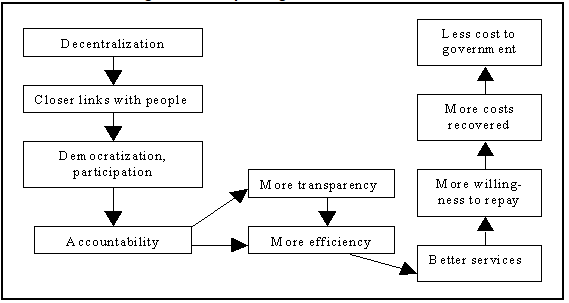
\includegraphics[width=0.8\textwidth]{Decentral.png}
    \caption{ Advantages of Decentralization of Governance }
    \label{fig:Advantages of Decentralization of Governance}
\end{figure}

% [image source - http://www.fao.org/docrep/005/y2006e/y2006e05.gif]

Consequently, the designed application will be used by the volunteers for the easy dispersal of information to the local people. People will remain informed about the ongoing government schemes, daily livelihood services and other local news. Participation in the ongoing surveys will also be managed and tracked easily. Delegation of community monitoring in the hands of volunteers will help in achieving the decentralization of governance effectively. 

\section{Literature Review and Related Work}
India is witnessing a phenomenal increase in mobile phone usage particularly in rural India over the last few years. Mobile handsets have become affordable and feature-rich making them amenable to value added applications. There is a consensus among mobile service providers, mobile content developers, banks and other financial institutions, policy makers (i.e., Reserve Bank of India, Ministry of Panchayat and Rural development), and various regulators (i.e., Telecom Regulatory authority of India, Indian Banks association, Insurance regulator of India, Mobile service provider association) that mobile applications is a viable way to reach information and service to rural people. The following papers were reviewed while developing the concept.

\begin{itemize}

\item Emergent Practices Around CGNet Swara, A Voice Forum for Citizen Journalism
in Rural India, ICTD’12 \cite{cgnet} : This paper talks about the initiative of CGNet Swara,
which is a project similar to JMR active in Chhatisgarh. The authors explain the
deployment of the system, and their experiences. It also delves into qualitative
and quantitative analysis of the data coming in, of the callers, topic about which
stories were reported among other things.

\item Designing Mobile Interfaces for Novice and Low-Literacy Users,ACM Transactions
on Computer-Human Interaction. 2011 \cite{design}: This study explores different interfaces
for low-literacy and novice mobile users. The authors conducted two studies com-
paring text-based interfaces to other different alternatives such as, one: automatic
solutions including graphics, spoken dialog and text-free user interfaces and sec-
ond: a live human operator. Based on these studies and interviews conducted
with the subjects, the authors cite results regarding the comfort of novice users
with the different mobile interface components. They also lay down certain design
recommendations while designing mobile user interfaces for such users.

\item Citizen Connect SMS Mobile Application \cite{Decen5:online} : This mobile application empowers citizens with access to information and grievance redressal of local government services.SMC was launched to provide latest information and facts to people and take the government services to the doorsteps of the citizens. They launched a mobile app ‘Citizens Connect’ that enables information sharing and service providing through latest technology.  The mobile app, which can be downloaded free of cost on Android phones, provides information regarding elected and administrative wings, registration procedures, recruitment advertisements and even rainfall. Users can also check birth and death certificate details, property tax details, pay water meter bills and share feedback. Having launched in 2013, the app has already received over 18 million service requests and 7400 complaints.


\item Mygaon, Web Platform \cite{MyGao25:online} : The initiative is centered around India’s 6.4 lakh villages, and more importantly, their efforts towards ensuring that each of native village is prosperous, healthy, and safe place to live. Mygaon's vision is to create a comprehensive, dynamic and interactive web platform of information on villages in India in order to facilitate impactful and accelerated social change.On My Gaon, one is able to browse through real-time information on villages in India in a rich and visual manner. One can also view information regarding verified organizations which are involved in successful and highly impactful projects in these locations. They introduce 'Village Champions' - individuals on the ground who are willing to help community people make a lasting impact in the villages and thus provide them with all the information, tools and networks one need to contribute to one's native village.

\item Rural ICT : Rural Information and Communication Technology (ICT) is a software platform that leverages cheap mobile phones and opportunistic Internet access for commercial purposes as well as group-based knowledge exchange. Users interact with the platform by dialing a phone number and navigating simple automated prompts using touchtone keys. It is a knowledge sharing system built for telephony, which empowers its users to engage in conversation, trade or exchange of ideas in any language and with any community, thus surmounting literacy and language challenges. The voice portal is a 24-hr system where customers can record their order any time, it will thus help in saving time, effort and money. Orders placed would be easily manageable, can be tracked and avoid any loss or missing orders. There is no limitation on no. of user availing this facility in a group and thus also can be used for public surveying. This automating of job is to set an online system - to process transactions and announcements.

There are three users of the system named as admins, publishers and the members. The customers register to the system as members. The publisher along with the permission of the admin will handle the system and broadcast messages to respective customers.The members of the system, the customers can place their request on the system. It may be in the form of an order, a feedback or a response. All their response and request will be stored in the system and the publisher or the admin will make sure that the order is being processed successfully. Thus with the help this system, one can record a message (special offers or notifications) to be broadcasted.

\item Comparing Semiliterate and Illiterate Users Ability to Transition from Audio+Text
to Text-Only Interaction, CHI’09 \cite{findlater2009comparing} : In this paper, the authors establish fact that
illiterate and semi-literate users can’t be both clubbed together into one category
when it comes to designing suitable user interfaces for them. This is so because for
users with some basic literacy, who though might not be able to read and write flu-
ently, text provides an unambiguous mode of interaction. The authors conducted
studies where they found that when semi-literate users were presented with an
interface with both text and audio support, they soon reduced their dependence
on audio while no such improvement was found in case of the fully illiterate users.
The paper provides interesting insights into the differences in the responses of fully
illiterate and semi-literate users to different UI components.
\end{itemize}




\chapter{Landscaping Study}

%Replace \lipsum with text.
% You may have as many sections as you please. This is just for reference.
Before building any technology, we must explore the existing technologies of the same doamin, their challenges and drawbacks, accessibility of these technologies to the target people and scalability issues. Many questions came in our mind before we started working on the solutions for information reachability to the community poeple.

\section {On Ground Surveys}
We conducted on ground surveys in the information deprived and backward areas of Delhi to find the answers of various questions. What type of problems are generally faced by these people? How people use media and mobile phones for solving their community level grievances? How people gain access to daily information, get their complaints solved, receive benefits of Governemnt schemes? How is government involved in solving these matters? How the grievances are amplified which forces government to solve the problems? We tried to find the answers of these questions by conducting following on ground surveys.

\begin{enumerate}
\item \textbf {Survey of ‘Munirka Village’}

Munirka is an urban area in South West Delhi, located near Jawaharlal Nehru
University (JNU) and Indian Institute of Technology Delhi (IIT Delhi)
Campuses \cite{Munir91:online}. Munirka is a village where development has started in early 1990’s.
The area is mostly dominated by the jaat community. We entered in a dealer’s shop
and asked about the village life, sarpanch and marginalized group in munirka.

Moreover, we found that the sarpanch of munirka himself lives in “Vasant Kunj”
and rarely visits his constituency. That was very disappointing part as he was not
at all involved in solving the problems faced by his people. He also gave us contact
number of vice-sarpanch “Bharat Singh” who lives in a nearby street in munirka.
He said “Munirka is no longer a village and the area was well developed where
everyone owns a smart phone and living a standard life. All shop owners were well
equipped with basic amenities. We also talked to some local shop owners on the
main street. The place was still following the village third-tier Panchayati Raj
System. Some points are summarized below.

\begin{enumerate}
\item It is now termed as an urban area but the place still follows the hierarchy of
sarpanch, vice-sarpanch and community people.
\item Shop owners were using TV as their source of information. Some youngsters
were listening to the radios for infotainment.
\item People owns the shop and had the information of their residence and their
area.
\item Almost many people owns the mobile phones.
\item Government involvement was very less in their grievances.
\end{enumerate}

\item \textbf {Survey of ‘Vasant Vihar’}

Our next visit was towards vasant vihar. Vasant Vihar is an exclusive
neighborhood located in the South West Delhi district of National Capital Territory
of Delhi. We had a visit to “coolie camp” situated in the same place. It is a slum area
where people were living in adverse conditions. There was no proper sanitation
facilities and no hygienic conditions. More than 3000 jhuggi-jhopdiyas, some pakke
makaans were agglomerated in such a small area. The irony is “Vasant Vihar is one
of the expensive residential areas in the world”  and it
still has such slum areas.\\

Well, we asked various questions to the residents of that place regarding the
availability of basic amenities. Whether they are able to avail the benefits of various
schemes, are able to solve their problems at community level, or by the involvement
of the MLA of their area “Parmila Tokas”. They said for the issues of water and
electricity availability, they approach to the MLA’s office to put their problems.
Sometimes, Officials or people from some department or ministry come to take
surveys for various statistics related to literacy rate, population count, number of
schools, toiletries etc but problems of local people are not addressed. They take
numbers and put it in records. One of the person standing near the retail shop said
that they make no efforts after the surveys, just take the figures that too improper
and report to higher authorities. People were reluctant in answering the questions and were uninterested in sharing
the stories and experiences they face and encounter.

\begin{enumerate}
\item  Women were dependent on male members of their family, were unaware of the community information and were carrying no mobile phones.
\item Youngsters were carrying the smart phones for receiving and making calls
and were using it generally for two applications i.e. Facebook and Whatsapp.
\item Local shop owners of the slum areas were carrying basic phones.
\item People aged between 40 to 60 were using phones mainly for gas booking
purposes and for receiving and making incoming and outgoing calls
respectively.
\item Youngsters wanted job related information.
\item No one was much concerned about health problems and health grievances.
\item People rely on words of their peers. Local people generally got informed from
mouth to mouth communication by their peers.
\item Shop owners are aware of their locality, its problems but have no smart
media and were seemed pre-occupied with their own local problems.
\end{enumerate}


\item \textbf {Survey of Seemapuri}
Seemapuri is mainly a rural zone in Delhi. New Seemapuri is situated at one end of north east Delhi. It has Uttar Pradesh as border on one side and lies adjoining to Dilshad Garden in East Delhi. It is basically a heterogeneous community with multi-cultural, multi-lingual and multi-characteristic features. Most of them earn their bread and butter by picking and sorting of rags. Some are daily wage earners, street vendors, domestic helps, and many other menial jobs which are the main stay of their sustenance. Few of them are also shopkeepers, rickshaw pullers and semi skilled labourers working in the construction sector. The fact remains that many of the families are unable to feed their children with the meagre earnings they make.
\begin{enumerate}
\item There are two slums near dilshad garden metro station, Rajeev camp and Sonia camp which were earlier displaced from some other area of Delhi to Dilshad garden due to ongoing construction.
\item Rag pickers earn their wages by picking and selling waste material which is too less for their livelihood.
\item No government surveillance and cleanliness of the locality is maintained.
\item People are poorly literate and have no source of information to participate in social development and governance related activities.
\end{enumerate}

\end{enumerate}


\section{Visit to NGOs}
A non-governmental organization (NGO) is a not-for-profit organization that is independent from states and international governmental organisations. They are usually funded by donations but some avoid formal funding altogether and are run primarily by volunteers. NGOs are highly diverse groups of organizations engaged in a wide range of activities, and take different forms in different parts of the world. We talked to NGO personnel of 'Action India' working in Seemapuri Area for the cause of community peopel and for solving their  community and livelihood problems. 
\begin{enumerate}
\item \textbf {Visit to Action india}
Action India founded in 1976, has taken many big and small path breaking initiatives by grassroots women, which clearly indicates the strong potential in women to become change agents in the process of social transformation. Action India sustains a balance between community based work and the universal struggle for women’s rights. While protesting against wrongs, Action India simultaneously creates alternative modes of self-help, self-esteem and self-assertion.

We had a talk with Mr. Praveen from Action India, project co-ordinator Mr. Deven
and Mr. Pramod regarding Action India's approach in solving problems of women
and various programs like 'Women helping women', 'Save the girl child campaign', 'Adolescents-Education for equality', 'Access to water and sanitation', 'Rural Program - looking through a gender less'. Various sanghs like 'Sable mahasangh maitreyi mela', 'Hinsa mukt mahilaye', 'Beti utsav' were started and are being run.

The NGO works for women empowerment program. We have discussed the ways they follow to solve the problems of women.

 \item \textbf{Cause of Action India}
\begin{enumerate} 
 \item   \textbf{Eliminate Discrimination} : Action India initiated the Mahila Panchayat (women’s courts) as a forum for
dispute resolution and realized need and effectiveness of women’s support groups. With the help of legal resource persons the paralegal workers trained the mahila panchayat members on legal rights of women with a strong focus on gender equality. Paralegal workers from the community, mobilized members for the mahila panchayats and today we have 9 mahila panchayats in Delhi. Mahila Panchayat has 14 paralegals and 225 mahila panchayat members. Mahila Panchayats themselves involve in solving the issues of women and support all the cases without any bias till the end.

 \item \textbf{Facilitate access to education} : For education related issues, they approach to School Management Committees, Dept. of School Education and Literacy, Ministry of Human Resource Development, Government of India which sometimes involve in solving the teacher absenteeism problem, School Mgmt Team, Mid day meal Distribution etc.
 
 \item \textbf{Facilitate access to health care} : They approach to health and sanitation committee where they force them to solve
the issues, go to deliver reports in person, for complaints they seek for constant reports and keep receiving to show in case they don’t entertain. NRHM benefits are also seeked by people.

 \item   \textbf {Enhance access to livelihood and economic rights} : Near the New Seemapuri Road which is approx. at 1 km distant from the Dilshad garden metro station, the complete road is occupied by the rag pickers (kabadi vala)
with their sacks. Due to this, this road smells very much and the residents have
problem with it. But as the Action India volunteer Mr. Praveen told us, this work is
the only livelihood for these rag pickers. Also, the MCD vehicle cleans all the
leftouts by the rag picker daily in the evening. We talked to the rag pickers also
asking the problems faced by them and how do they get it solved. We found from the
conversation that their voice is not heard by anybody nor it is communicated to the
govt. authorities.
When they were told about the android application features, they found the
grievance redressal the most useful. As their primary need is to secure their
livelihood and not the secondary needs which they cannot even think to access.
 \item  \textbf{ Enable participation in governance and development} : They encourage people to participate in the local governance related and development issues of society.
\end{enumerate}

\end{enumerate}




\section {Observations and Suggestions}

\begin{enumerate}
\item Political Agenda for all the commissions matters more than the actual solution for the problem.
\item School Association Committee (SMCs), health and sanitation committee (HSC) were not able to solve and address the villagers problem effectively.
\item Recognizing and delivering on-ground training to Human Access Points.
\item Unawareness of HAPs regarding local community problems
\item Data Security and Multi-lingual Support
\item On –ground training is mandatory before launching any scheme, giving any
benefits, introducing ICTD media among people, deploying any technology.
\item Manual intervention and involvements are the key elements in introducing
big changes and turning heads of the people.
\item The local knowledge of village is very important prior introducing any new
model in that place.
Necessity of responsible people in various regulatory authorities, commission
departments, panchayats, Government officers, NGO’s workers, ASHA
workers, school teachers.
\item People should themselves come forward to seek solutions and seek
information and registering complaints.
\item Mobile phones users are many and they can be given on ground training for
making the human access points and local villagers known with the problem
and the technologies.
\end{enumerate}

\section {Conclusions}
It is analysed from all the surveys that people who live in the underdeveloped areas
like rural areas and the slums do not have a platform where they can get all theinformation about the basic needs which they require in their lifestyle. Information
about administration, education, health schemes, employment, agriculture, gas
cylinder bookings, land acquisitions can be correctly communicated to them which
will help them on fulfilling their needs and eventually develop and making their
lifestyle better. But there are certain problems in the implementation of the
method.

\begin {enumerate}
\item  People do not have even small knowledge of operating the mobile phones
whether basic mobile phones or smart phones. Condition is even worse with
women. Though youth and earning member of the house have phones but
still they do not know more than dialing and receiving the call thus intense
training is required for the proper implementation of the approach.
\item  People are reluctant in sharing the information to the people outside their
community. Or they tell data which is partially or completey false. Thus to
collect data through telephonic surveys, Trust needs to be built that it is for
their welfare only.
\item If started by implementing the approach for all the areas mentioned above, it
is unlikely that it will be implemented properly for all the fields and a large
dataset of information is required and need to be maintained. Thus the
approach should be started by implementing for 1 or 2 areas initially.
\end {enumerate}



\chapter{System Architecture}

\section{Technologies Used}
\subsection{Platform and Technologies - Application Server / Web Server}
\begin{itemize}
  \item Implemented using Ruby on Rails web framework \cite{Ruby}
  \item Database is designed using MySQL
  \item GCM Server
\end{itemize}

\subsection{Application Design}

\begin{itemize}
\item Android Platform with Android Studio 1.1.0 \cite{Intro42:online}
\item Database is designed using SQLite.
\item Using Volley Libraries for asynchronous task communication to the network server \cite{Andro34:online}
\item Android 5.0.1 Minimum SDK build tool and Platform tool with APIs level 21 or above support
\item GCM Client
\end{itemize}

\section{System Flow}

Following Diagram depicts the entire System Flow.
\begin{figure}[H]
    \centering
	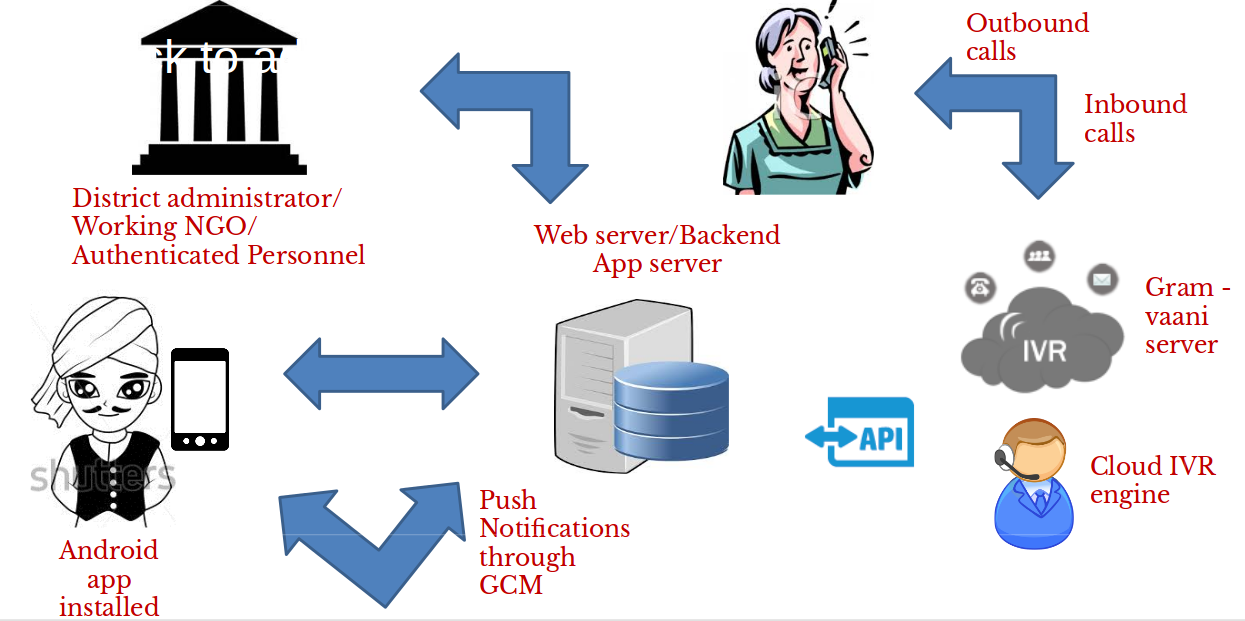
\includegraphics[width=0.8\textwidth]{Sysflow.png}
    \caption{System Flow}
    \label{fig:System Flow}
\end{figure}

\section{Use Case Diagram}
\begin{figure}[H]
    \centering
	\includegraphics[width=0.8\textwidth]{UseCaseDiagram.png}
    \caption{Use Case Diagram of Application User}
    \label{fig:Use Case Diagram of Application User}
\end{figure}

\section{Class Diagram}
\section{ERD Schema}
\section{Information flow}
Mobile Application is designed for the volunteers of the village. Along with, a portal is designed for the  NGOs/ Block or district officials for sending alerts to the volunteers of the community. Some volunteers from the community ( For instance, panchayat members, School teachers) will be chosen by the functioning NGO or block/ district administrator under which the community/ village falls. NGOs/ Block or district officials will give authorization to the selected volunteers from that community by registering them through the portal. After authorization, volunteers will be given an Android phone pre-loaded with the local governance application “ Gologo”. Credentials of volunteers will be authenticated on first time login in the application. After successful one time login, volunteers aid their local community people by exploring the app functionalities. Portal will be used to send survey alerts to the volunteers. Volunteers will receive alerts  on their mobile phones to further disperse it to the target people. Through this way, information will flow by the people and  among the people via following functionalities.

Following diagram depicts the functionalities provided to the app user.

\begin{figure}[H]
    \centering
	\includegraphics[width=10cm,height=10cm,keepaspectratio]{Workflowapp.png}
    \caption{Functionalities of Application User}
    \label{fig:Functionalities of Application User}
\end{figure}

Following Diagram depicts the flow of information through \hyperref[itm:launchsur]{Launch Survey Use Case} whcih is explained later.

\begin{figure}[H]
    \centering
	\includegraphics[width=0.9\textwidth]{launchsurvey1.png}
    \caption{Launch Survey Use Case}
    \label{fig:Launch Survey Use Case}
\end{figure}


\chapter{Gram Vaani APIs Communication}

\begin{enumerate}
\item
Usage : The API is called to fetch the locations saved in gram vaani database.

Details / Hacks : From response, desc value having state, district and block is displayed in list view. State-District-Block is split from the desc parameter and sent to the server as key value post params <state> : <value>, <district> : <value>, <block> : <value>, <resource
_uri> : <value> to save under respective columns in app database.


\chapter{Gram Vaani APIs Communication}
Following GV APIs are used to achieve the functionalities given to the end users and NGO personnel.
 
\section{Launch and View Surveys}
\begin{itemize}
\item Get Active Surveys : To get the surveys of a particular app\_instance
\ \\
API URL : /survey\_survey/
\item Get Survey Questions : To get the form of a survey, which contains the questions.
\ \\
API URL : /form\_question/

\item Get Responses : To get the responses of a survey.
\ \\
API URL : /survey\_record/cdr\_records/

\item Create Questions : To create questions for a particular form. The responses to the questions can be of three type Voice\/MCQ\/Quantitative
\ \\
API URL : /form\_question/add/
\item Upload Audio : To upload audio prompts, which can be used later as a question\/prompt
\item Create Survey : After creating the form\_questions, the survey needed to be saved. This will make the survey active by default.
\  \\
API URL : /survey\_survey/save/

\end{itemize}

\section{Contact Groups Management}
\begin{itemize}
\item Get Contact Lists\/Groups : Fetches all the contact groups (lists) maintained by the user.
\ \\
API URL : /callerinfo\_contact\_list/

\item Get Contacts : To get the contacts of a particular contact list
\ \\
API URL : /callerinfo\_contact/
\item Create New Contact List : To create a new contact list in GV instance
\ \\
API URL : /callerinfo\_contact\_list/
\item Create Contact in Single or Multiple Contact Groups : To create a new contact and adding it to multiple contact\_lists
\ \\
API URL : /callerinfo\_contact/
\end{itemize}


\section{Audio Broadcast}
\begin{itemize}
\item Create New Item : It helps in creating a new item on the GV server. Creating an item instance on mnews returns instance id which will be used to upload audio on the GV server.
\ \\
API URL : mnews\_news /create\_new\_item/
\item Upload Audio : MNEWS API will be called to upload an audio and make it as a news item's recording.
\ \\
API URL : mnews\_news\/upload\_audio\/
\item Uploading on Default Channel : To upload audio by getting the default channel of the app instance.
\ \\
API URL : /media\_prompt\_audio/upload\_audio/
\end{itemize}

\newpage
\section{Message Broadcast}
\begin{itemize}
\item Sending Message : Message will be sent in the form of template with various template parameters along with the target contact list.
\ \\
API URL : sms\_message/send/
\item Check Message Status : sms\_message with GET request along with app instance ID can be used to check the status of message delivery for a particular caller ID.
\ \\
API URL : /vapp/api/v1/sms\_message/id
\end{itemize}

\ \\

Note - Base URL : http://internal.gramvaani.org:8080/vapp/api/v1


\chapter{Results}

\section{Screenshots of the Application Interface}

\begin {enumerate}
\item First time app Users will be authenticated via PIN received through the message on NGO Registration.
\begin{figure}[here]
\begin{center}   
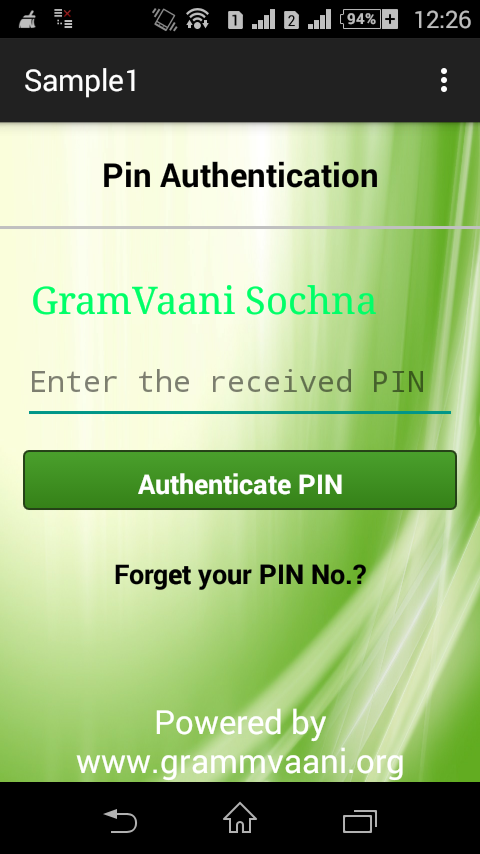
\includegraphics[scale=0.3]{pin_authenticate}
\caption{Pin Authentication}
\label{fig:pin_authenticate}
\end{center}
\end{figure}

\item Online User Registration by the NGO sends a message on registered number for authentication.
\begin{figure}[here]
\begin{center}   
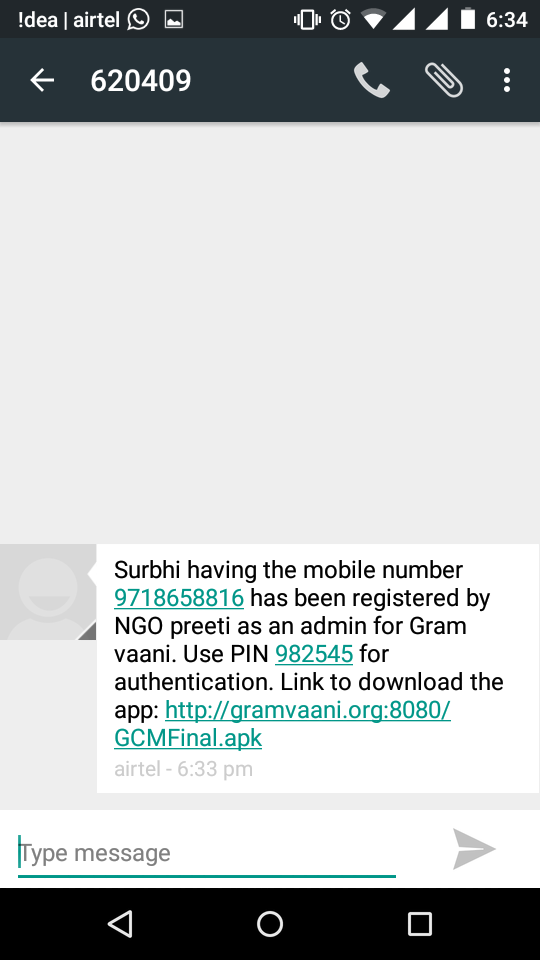
\includegraphics[scale=0.3]{authenticatemsg}
\caption{Message for Pin Authentication}
\label{fig:authenticatemsg}
\end{center}
\end{figure}

\item User can retrieve PIN by clicking on Forget PIN option.
\begin{figure}[here]
\begin{center}   
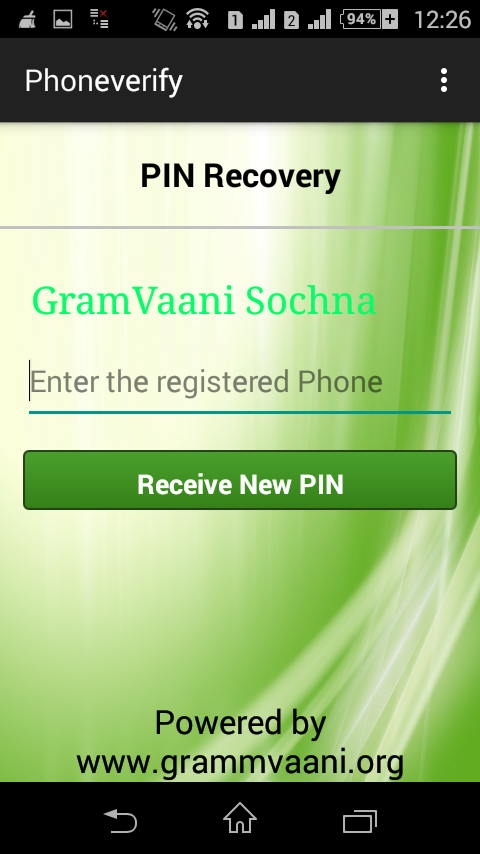
\includegraphics[scale=0.3]{pin_recovery}
\caption{Pin Recovery}
\label{fig:pin_recovery}
\end{center}
\end{figure}

\item User will be provided with the following options.
\begin{figure}[here]
\begin{center}   
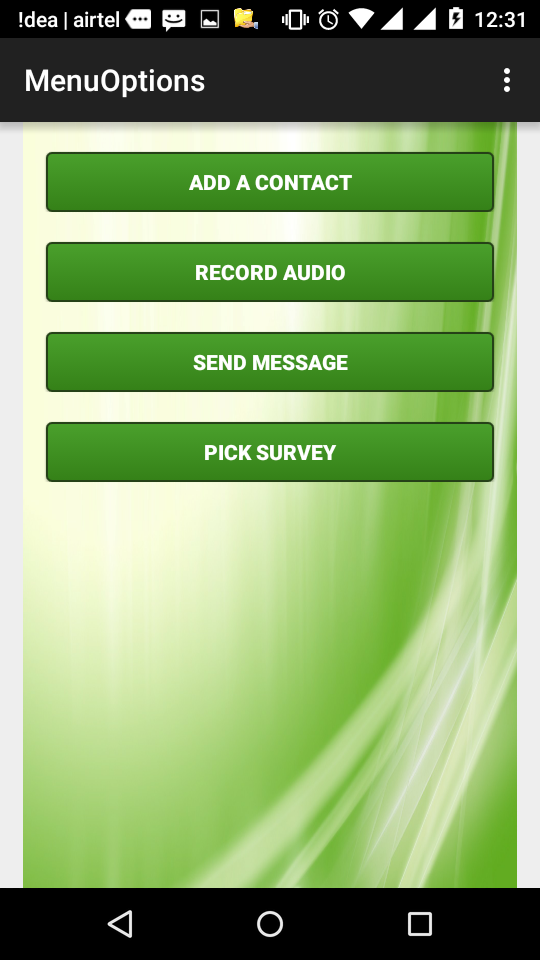
\includegraphics[scale=0.3]{menuoptions}
\caption{Use Cases}
\label{fig:menuoptions}
\end{center}
\end{figure}

\item User can record audio by choosing audio format.
\begin{figure}[here]
\begin{center}   
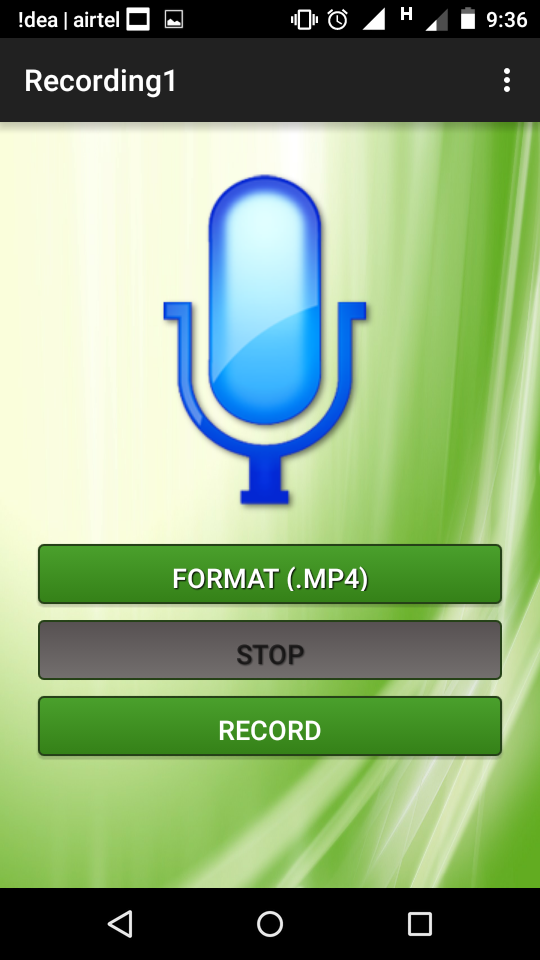
\includegraphics[scale=0.3]{audio1}
\caption{Record Audio}
\label{fig:audio1}
\end{center}
\end{figure}

\item User can choose to either save\/send\/discard an audio message.
\begin{figure}[here]
\begin{center}   
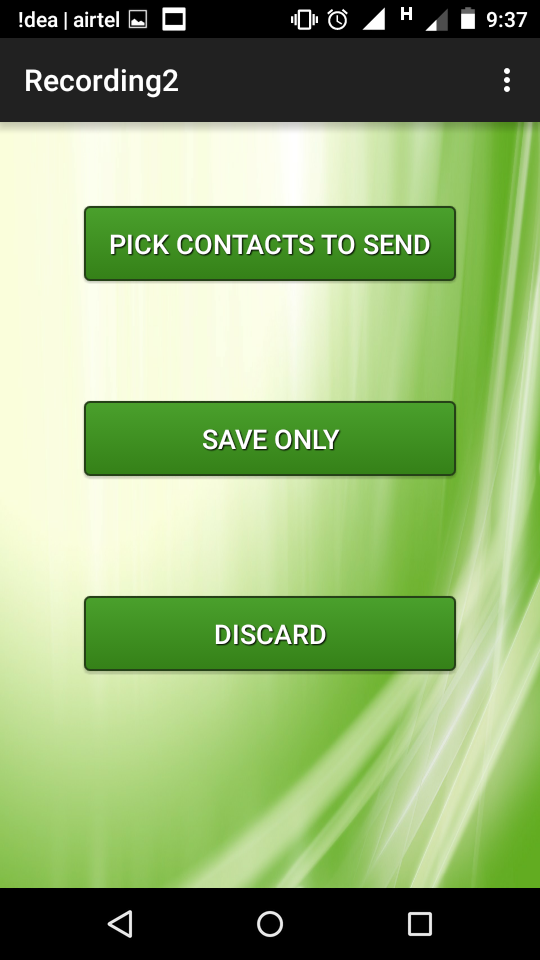
\includegraphics[scale=0.3]{audio2}
\caption{Options After Recording Audio}
\label{fig:audio2}
\end{center}
\end{figure}

\item User can speak a message or type the message to send.
\begin{figure}[here]
\begin{center}   
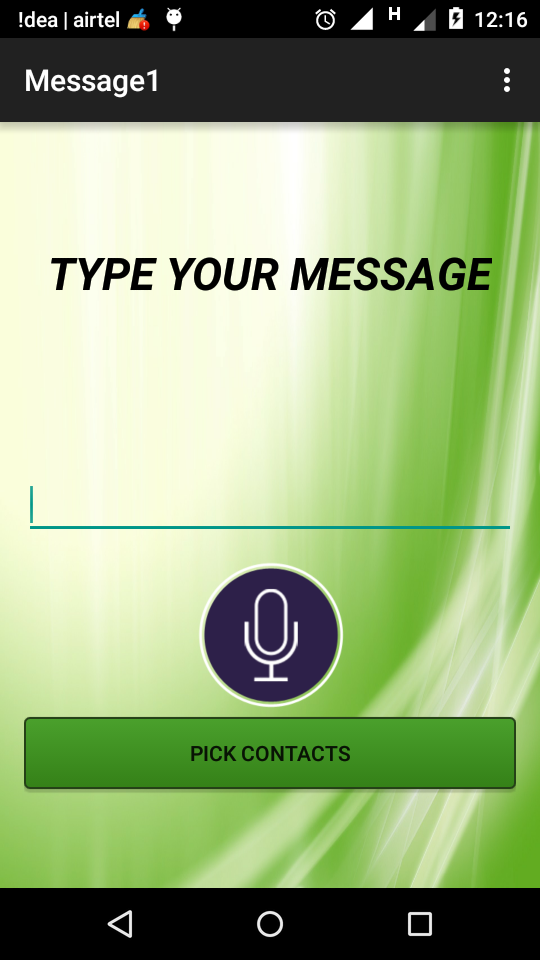
\includegraphics[scale=0.3]{msg1}
\caption{Speak/Type Message}
\label{fig:msg1}
\end{center}
\end{figure}

\item User can view all the active survey names of the GramVaani Server.
\begin{figure}[here]
\begin{center}   
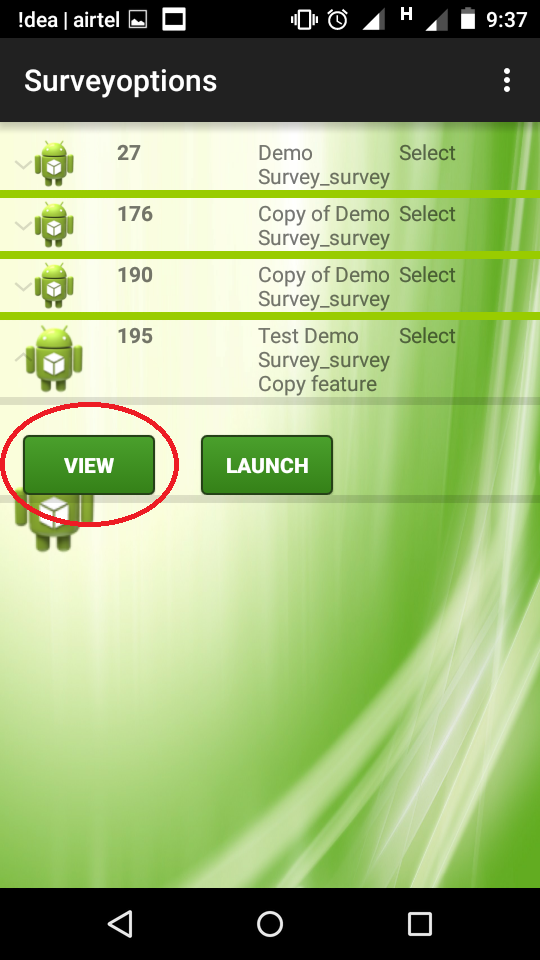
\includegraphics[scale=0.3]{viewlaunchsurvey}
\caption{List of Active Surveys}
\label{fig:viewlaunchsurvey}
\end{center}
\end{figure}

\item User can view a particular survey with all survey questions on selection.
\begin{figure}[here]
\begin{center}   
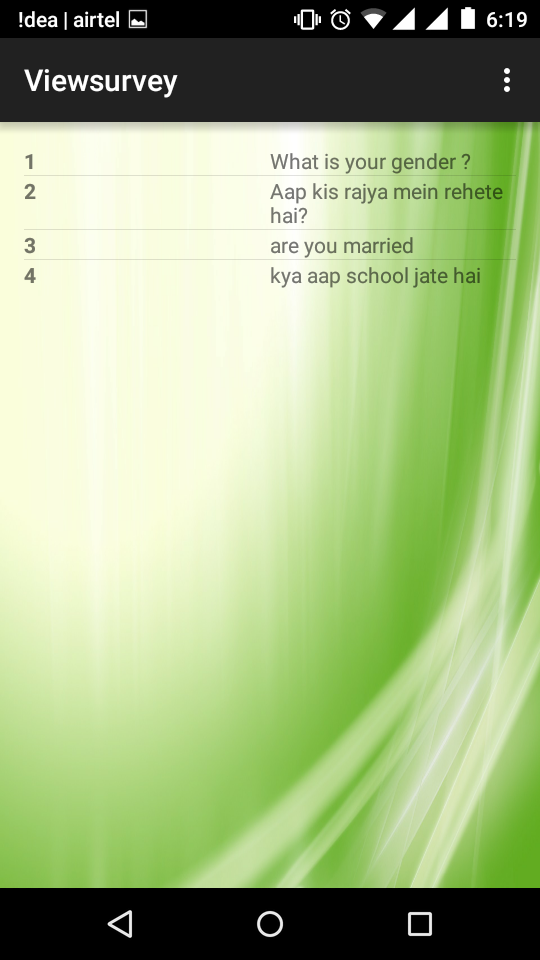
\includegraphics[scale=0.3]{viewsurvey}
\caption{View a Particular Survey}
\label{fig:viewsurvey}
\end{center}
\end{figure}

\item User can choose the target people among his phone callers, GV callers, Mobile Vaani Recent Callers and GV groups.
\begin{figure}[here]
\begin{center}   
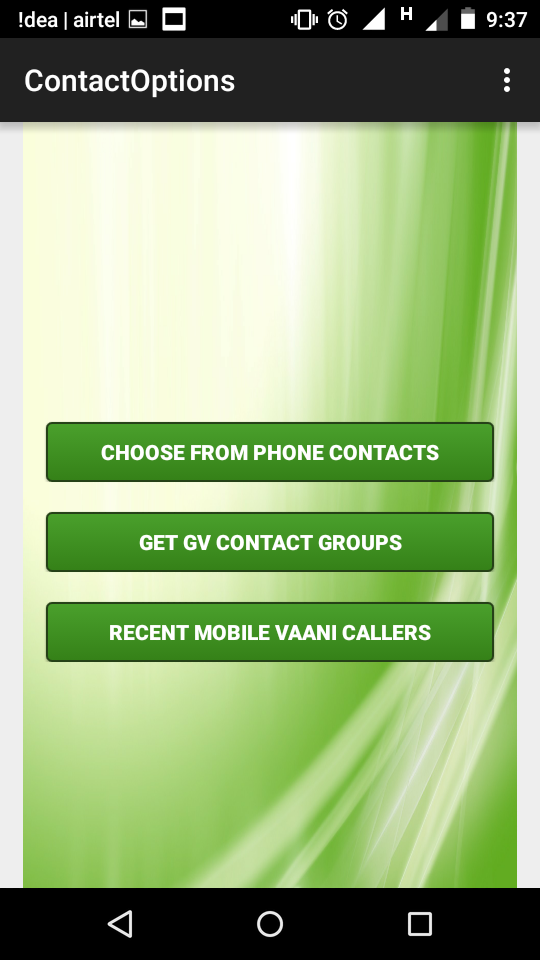
\includegraphics[scale=0.3]{contactoptions}
\caption{Choose Target Contacts}
\label{fig:contactoptions}
\end{center}
\end{figure}

\item Multiple GV contact groups can be choosen as the target people.
\begin{figure}[here]
\begin{center}   
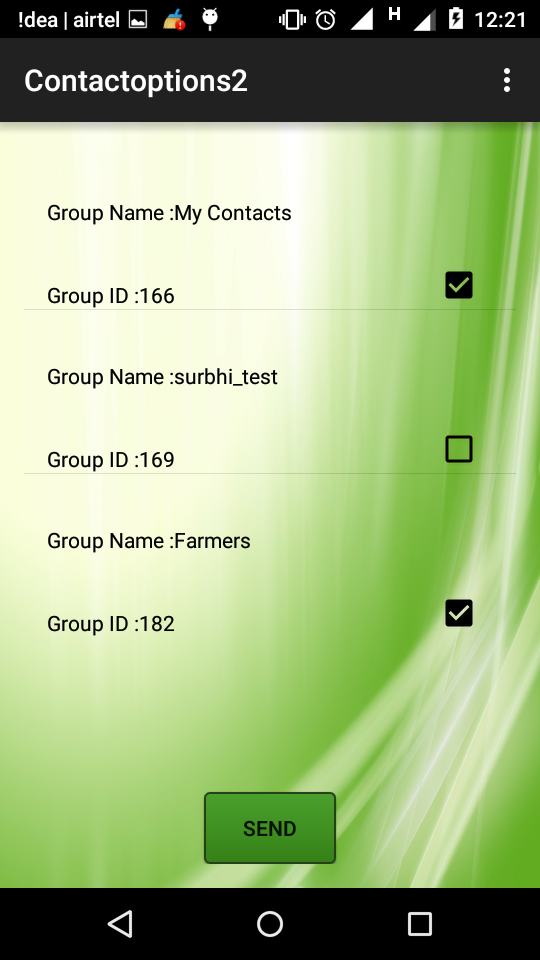
\includegraphics[scale=0.3]{contactgroups}
\caption{GV Contact Groups}
\label{fig:contactgroups}
\end{center}
\end{figure}

\item Multiple phone contacts can be choosen as the target people.
\begin{figure}[here]
\begin{center}   
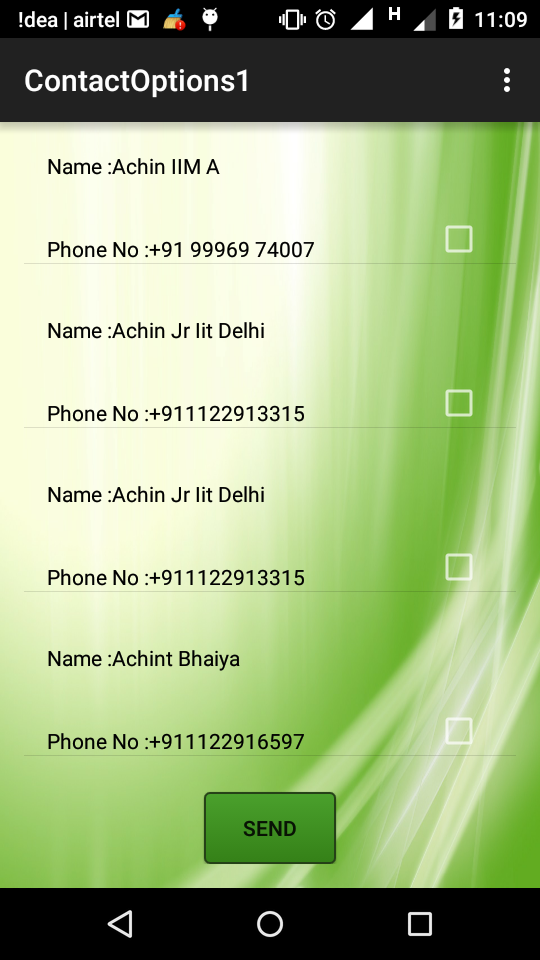
\includegraphics[scale=0.35]{phonecontacts}
\caption{Phone Contacts}
\label{fig:phonecontacts}
\end{center}
\end{figure}

\end{enumerate}

\section{Screenshot of the GramVaani Web Instance}

\begin{enumerate}

\item GramVaani Graphical Web Portal Instance
\begin{figure}[here]
\begin{center}   
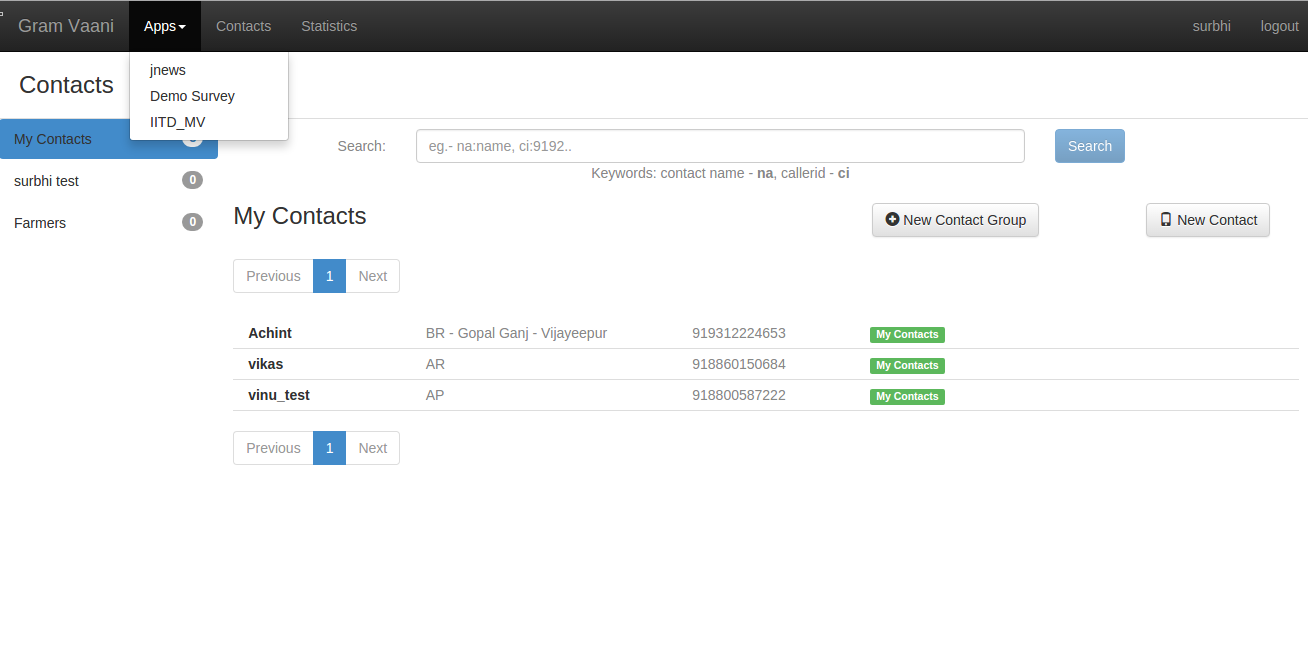
\includegraphics[scale=0.3]{gvinstance1}
\caption{GramVaani Web Instance}
\label{fig:gvinstance1}
\end{center}
\end{figure}


\end{enumerate}




\section{Screenshots of the Web Portal}

\begin{enumerate}
\item Home Page of the Web Portal for NGO's Registration and other functionalities
\begin{figure}[here]
\begin{center}   
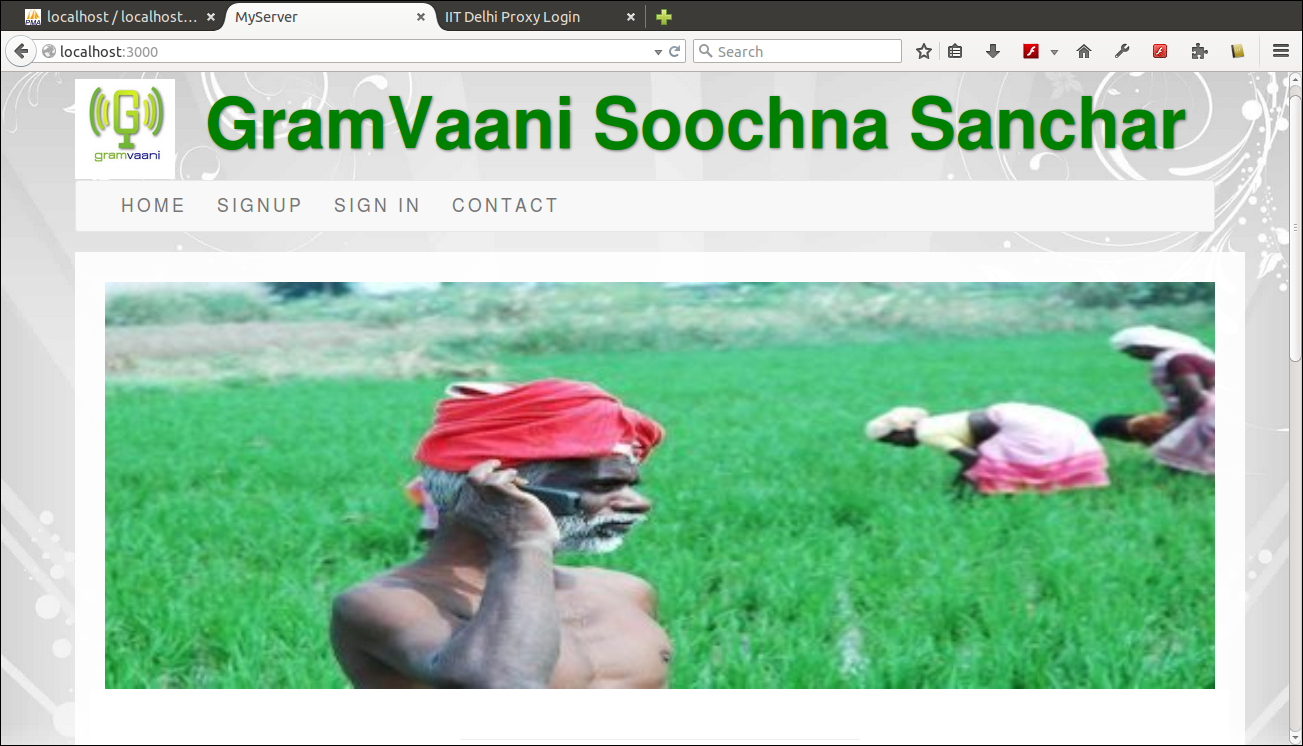
\includegraphics[scale=0.3]{w1}
\caption{GramVaani Soochna Sanchar Home Page}
\label{fig:w1}
\end{center}
\end{figure}


\item NGO's Login Page
\begin{figure}[here]
\begin{center}   

\includegraphics[scale=0.3]{w10}
\caption{NGO's Login Page}
\label{fig:w10}
\end{center}
\end{figure}



\item Use cases provided to the NGO users
\begin{figure}[here]
\begin{center}   

\includegraphics[scale=0.3]{w14}
\caption{Use Cases of NGO Personnel}
\label{fig:w14}
\end{center}
\end{figure}



\item Web Online form for Admins Registration and Authentication
\begin{figure}[here]
\begin{center}   
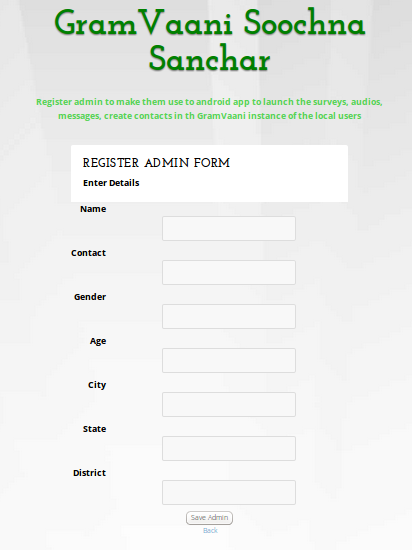
\includegraphics[scale=0.3]{w15}
\caption{Admin's Registration Form}
\label{fig:w15}
\end{center}
\end{figure}




\item NGO Personnel can launch a particular survey for a particular district.
\begin{figure}[here]
\begin{center}   
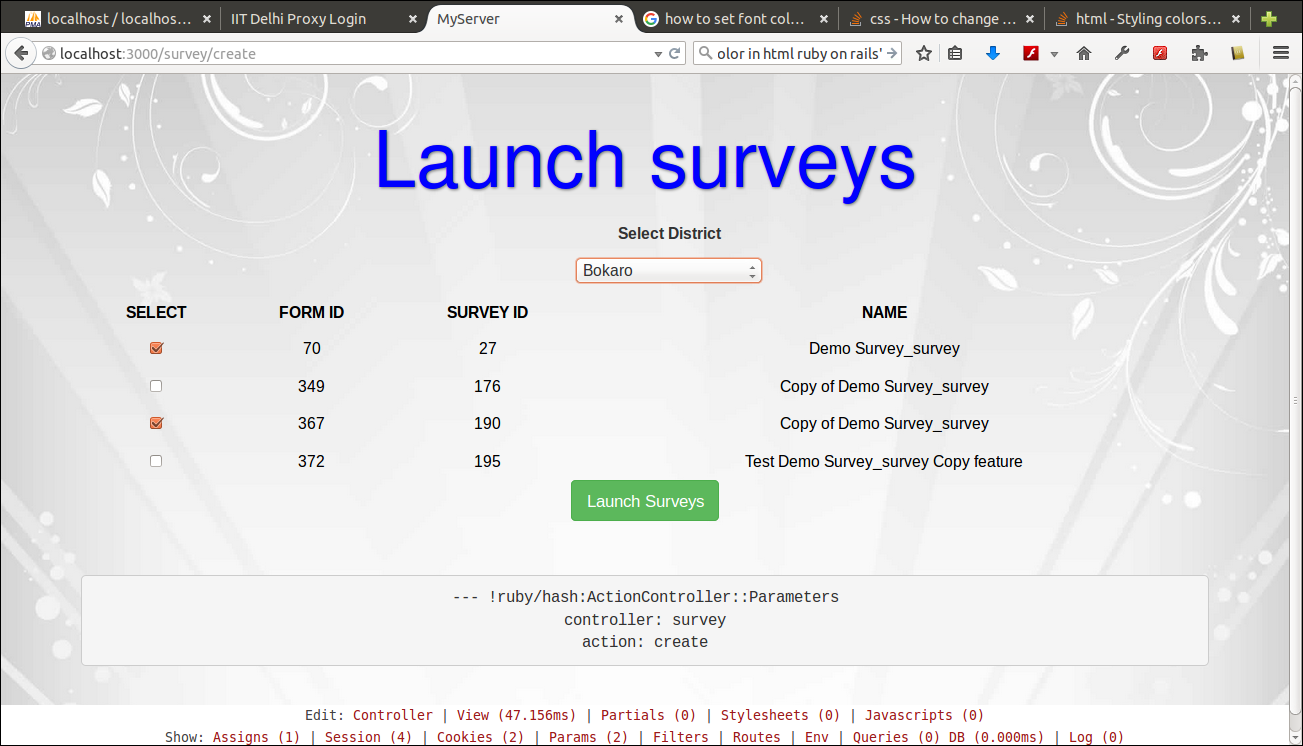
\includegraphics[scale=0.3]{w16}
\caption{Launch Survey in a District}
\label{fig:w16}
\end{center}
\end{figure}


\item NGO Personnel can view all the active surveys along with viewing current responses and survey questions.
\begin{figure}[here]
\begin{center}   
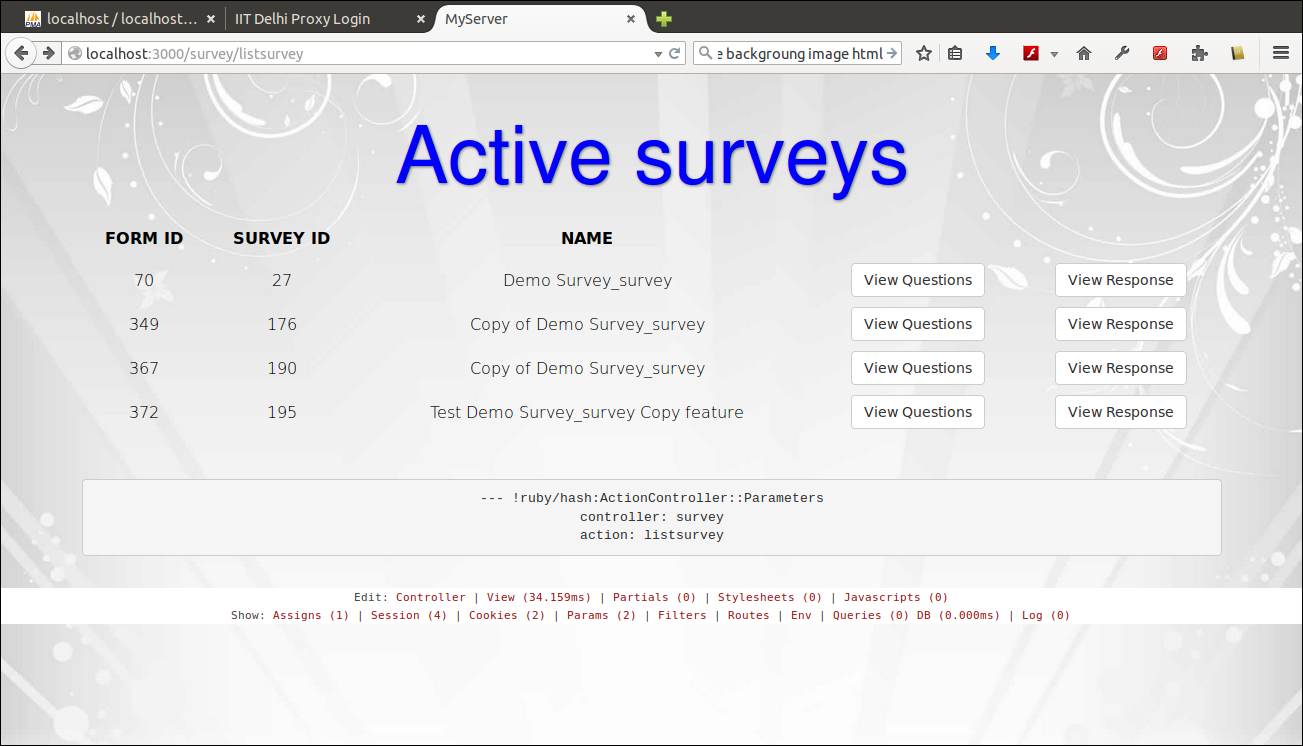
\includegraphics[scale=0.3]{w13}
\caption{View Active Surveys}
\label{fig:w13}
\end{center}
\end{figure}


\item NGO Personnel can view the responses of the active survey.
\begin{figure}[here]
\begin{center}   
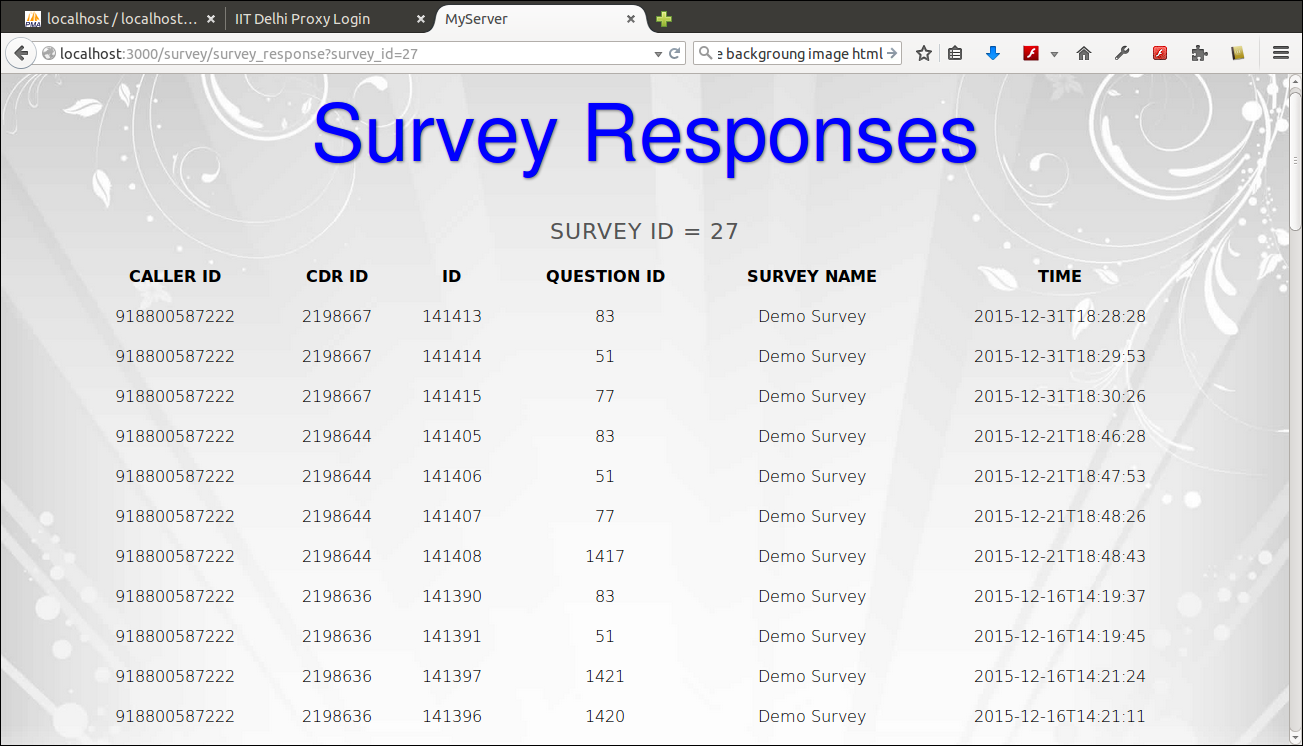
\includegraphics[scale=0.3]{w11}
\caption{View Active Survey Responses}
\label{fig:w11}
\end{center}
\end{figure}


\item NGO Personnel can view the text questions of the active survey.
\begin{figure}[here]
\begin{center}   
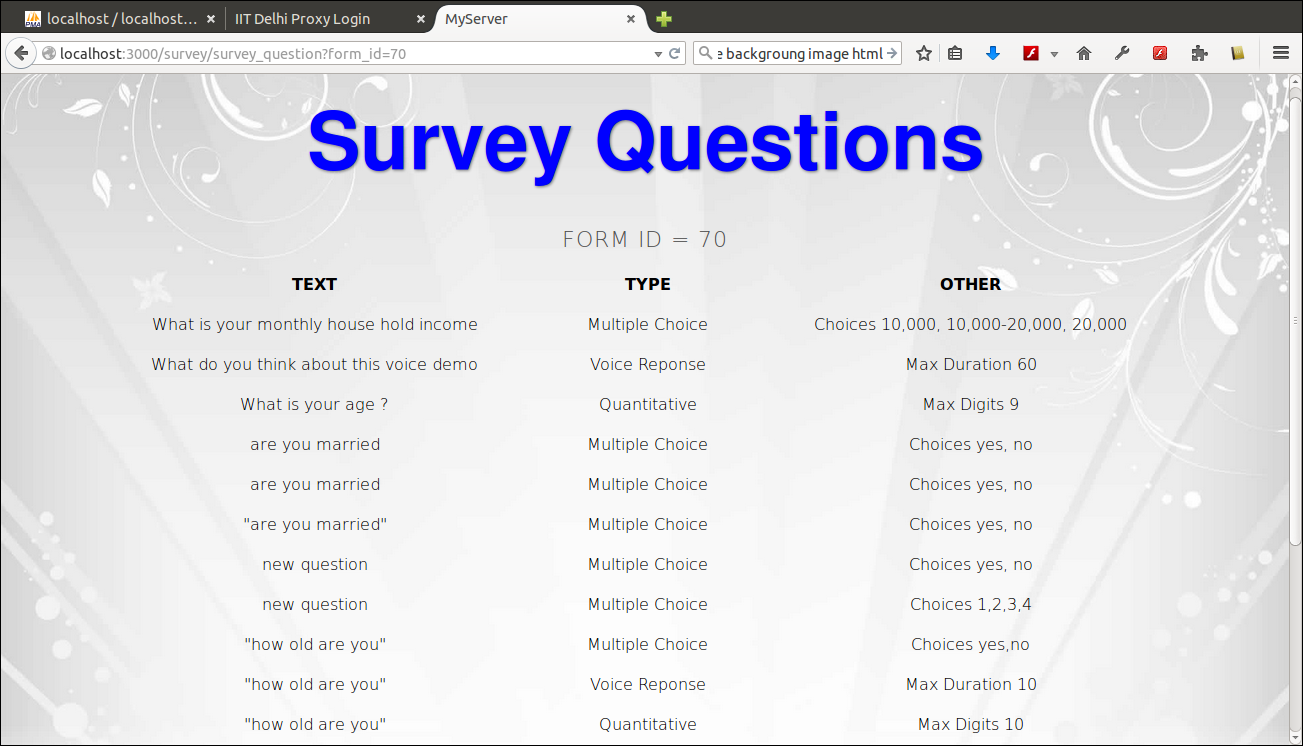
\includegraphics[scale=0.3]{w12}
\caption{View Active Survey Questions}
\label{fig:w12}
\end{center}
\end{figure}
 
\end{enumerate}















\chapter {Google Cloud Messaging}
\section{What is GCM?}
\label{sec:gcmlink}
Google Cloud Messaging (GCM) is a free service that helps Android developers to send data from servers to their Android applications, and upstream messages back to the cloud from the user’s device. This can be a lightweight message telling the Android app that there is a new data to be fetched from the server or it can be a message containing up to 4Kb of payload data. The GCM service handles all the aspects of queuing of messages and delivery to the target Android application running on the target device.

\section{Characteristics of GCM}
\begin {enumerate}

\item    Allows 3rd-party application servers to send messages.
\item  Using GCM Cloud Connection Server, one can receive upstream messages from the user’s device.
\item Android application doesn’t need to be running on a device to receive messages. When the message arrives, system will wake up the Android application via Intent broadcast, as long as the application is set up with the proper broadcast receiver and permissions. Gologo uses WakefulBroadcastReceiver to awake the device when notofication arrives.
\item Built-in user interface or other handling for message data is not available, GCM simply passes raw message data straight to the Android application that has full control of how to handle it. For instance, survey alerts are sent and handled at the application side.
\item Requires devices running Android 2.2 or higher with Google Play Store app installed or an emulator running Android 2.2 with Google APIs.

\end {enumerate}

\section{GCM System Architecture}

\begin{figure}[H]
\begin{center}   
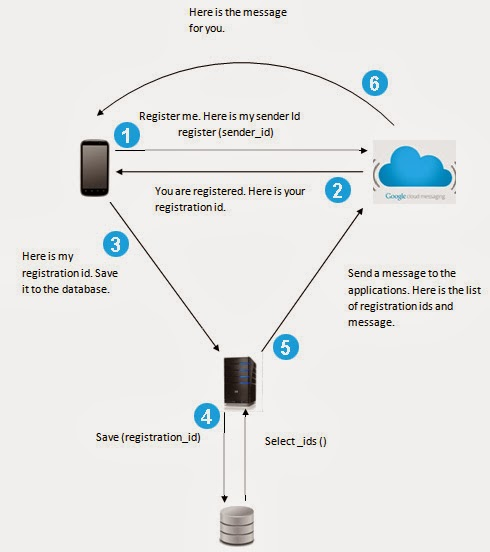
\includegraphics[scale=0.8]{GCM}
\caption{GCM System Architecture}
\label{fig:GCM}
\end{center}
\end{figure}

\section {Key Concepts of GCM}

\subsection {GCM Components}
\begin {enumerate}
  \item\textbf { Client App} – It is a GCM-enabled Android application running on a device. This must be 2.2+ Android OS device with Google Play Store installed, and it must have at least one logged in Google account if the device is running a version lower than Android 4.0.4.

   \item\textbf { 3rd party Application Server }– An application server that you write as part of implementing GCM. The 3rd-party application server sends data via the GCM connection server to Android application on the device.

    \item\textbf {GCM Connection Server} – These are Google-provided servers involved in taking messages from the 3rd-party application server and sending them to the device.

\end {enumerate}

\subsection {GCM Credentials}
\begin {enumerate}
  \item\textbf {Sender ID} – The sender ID is used in the registration process to identify a 3rd-party application server that is permitted to send messages to the device.

    \item\textbf{Application ID} – The Android application that is registering to receive messages.

    \item\textbf {Registration ID } – An ID issued by the GCM servers to the Android application that allows it to receive messages. Once the Android application has the registration ID, it sends it to the 3rd-party application server, which uses it to identify each device that has registered to receive messages for a given Android application.
    
 \item\textbf {    Sender Auth Token} – An API key that is saved on the 3rd-party application server that gives the application server authorized access to Google services. The API key is included in the header of POST requests that send messages.
\end {enumerate}

\section{Life Cycle Flow}
\begin{enumerate}
   \item\textbf {Enable GCM} – Android application running on a mobile device registers to receive messages. To use the messaging service on Android application for the first time, it needs to call the GoogleCloudMessaging method register(). The register() method returns a registration ID which should be stored by our Android application for later use.
   
   \item\textbf {Send A Message} – A 3rd-party application server sends messages to the device. Here is the sequence of events that occurs when the application server sends a message. Message is sent to GCM servers by the application server. Google enqueues and stores the message incase the device is offline. When the device is online, Google sends the message to the device. On the device, the system broadcasts the message to the specified Android application via Intent broadcast with proper permissions, so that only the targeted Android application gets the message. This wakes the Android application up. The Android application does not need to be running beforehand to receive the message. 
   
   The Android application processes the message. If the Android application is doing non-trivial processing, you may want to grab a PowerManager WakeLock and do any processing in a service. The Android application extracts the raw data from the com.google.android.c2dm.intent.RECEIVE Intent by key and processes the data.
        
   \item\textbf {Receive A Message} – Android application receives a message from GCM server. This is the sequence of events that occurs when an Android application installed on a mobile device receives a message.
   
   \begin{enumerate}
      \item  The system receives the incoming message and extracts the raw key/value pairs from the message payload, if any.
      \item The system passes the key/value pairs to the targeted Android application in a com.google.android.c2dm.intent.RECEIVE Intent as a set of extras.
   \end{enumerate}



\end{enumerate}


\chapter{Epilogue}


\section{Challenges}
Deployment may face the below listed challenges.
\begin{itemize}
\item Multi-Lingual support
\item Designing in coherence with end user capabilities
\item Capturing user requirements
\item Content Management and Content Moderation
\item Unawareness of HAPs regarding community problems.
\item Data Security
\item Scalability
\end{itemize}

\section{Conclusion}

\begin{enumerate}
\item On –ground training is mandatory before launching any scheme, giving any
benefits, introducing ICTD media among people, deploying any technology.
\item Manual intervention and involvements are the key elements in introducing
big changes and turning heads of the people.
\item The local knowledge of village is very important prior introducing any new
model in that place.
\item Necessity of responsible people in various regulatory authorities, commission
departments, panchayats, Government officers, NGO’s workers, ASHA
workers, school teachers.
\item People should themselves come forward to seek solutions and seek
information and registering complaints.
\item Mobile phones users are many and they can be given on ground training for
making the human access points and local villagers known with the problem
and the technologies.
\item Main issues and problems are specific to the villages, to the regions. They
need to be identified and then application can be used and make a great
contribution in actually helping people by various means.
\item For each department, there are separate commissions and agencies working
under them, they can be directly put in link with the problem.

\end{enumerate}
\section{Future Work}

\begin{itemize}
\item Introducing flexibility in user interface by minimizing user input
\item Sending push notifications and current status of scheduled task to app users through GV call-back APIs.
\item User Feedback and Real time Application Deployment
\item Dispatching information among NGO personnel and Application users 
\end{itemize}

\chapter {Google Cloud Messaging}
\section{What is GCM?}
Google Cloud Messaging (GCM) is a free service that helps Android developers to send data from servers to their Android applications, and upstream messages back to the cloud from the user’s device. This can be a lightweight message telling the Android app that there is a new data to be fetched from the server or it can be a message containing up to 4kb of payload data. The GCM service handles all the aspects of queuing of messages and delivery to the target Android application running on the target device.

\section{Characteristics of GCM}
\begin {enumerate}

\item    Allows 3rd-party application servers to send messages.
\item  Using GCM Cloud Connection Server, one can receive upstream messages from the user’s device.
\item Android application doesn’t need to be running on a device to receive messages. When the message arrives, system will wake up the Android application via Intent broadcast, as long as the application is set up with the proper broadcast receiver and permissions. Gologo uses WakefulBroadcastReceiver to awake the device when notofication arrives.
\item Built-in user interface or other handling for message data is not available, GCM simply passes raw message data straight to the Android application that has full control of how to handle it. For instance, survey alerts are sent and handled at the application side.
\item Requires devices running Android 2.2 or higher with Google Play Store app installed or an emulator running Android 2.2 with Google APIs.

\end {enumerate}

\section{ System Architecture}

\begin{figure}[here]
\begin{center}   
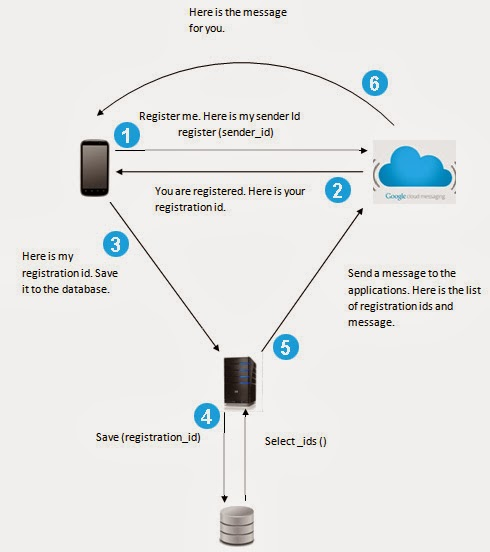
\includegraphics[scale=0.3]{GCM}
\caption{GCM System Architecture}
\label{fig:GCM}
\end{center}
\end{figure}

\section {Key Concepts of GCM}

\subsection {GCM Components}
\begin {enumerate}
  \item\textbf { Client App} – It is a GCM-enabled Android application running on a device. This must be 2.2+ Android OS device with Google Play Store installed, and it must have at least one logged in Google account if the device is running a version lower than Android 4.0.4.

   \item\textbf { 3rd party Application Server }– An application server that you write as part of implementing GCM. The 3rd-party application server sends data via the GCM connection server to Android application on the device.

    \item\textbf {GCM Connection Server} – These are Google-provided servers involved in taking messages from the 3rd-party application server and sending them to the device.

\end {enumerate}

\subsection {GCM Credentials}
\begin {enumerate}
  \item\textbf {Sender ID} – The sender ID is used in the registration process to identify a 3rd-party application server that is permitted to send messages to the device.

    \item\textbf { Application ID} – The Android application that is registering to receive messages.

    \item\textbf { Registration ID } – An ID issued by the GCM servers to the Android application that allows it to receive messages. Once the Android application has the registration ID, it sends it to the 3rd-party application server, which uses it to identify each device that has registered to receive messages for a given Android application.
    
 \item\textbf {    Sender Auth Token} – An API key that is saved on the 3rd-party application server that gives the application server authorized access to Google services. The API key is included in the header of POST requests that send messages.
\end {enumerate}

\section {LifeCycle Flow}
\begin {enumerate}
   \item\textbf {Enable GCM} – Android application running on a mobile device registers to receive messages.
    \item\textbf {Send A Message} – A 3rd-party application server sends messages to the device.
   \item\textbf {Receive A Message} – Android application receives a message from GCM server.
\end {enumerate}

\begin {enumerate}
\item\textbf {Enable GCM}
To use the messaging service on Android application for the first time, it needs to call the GoogleCloudMessaging method register(). The register() method returns a registration ID which should be stored by our Android application for later use.

   \item\textbf { Send A Message} : Here is the sequence of events that occurs when the application server sends a message.
        Message is sent to GCM servers by the application server.
        Google enqueues and stores the message incase the device is offline.
        When the device is online, Google sends the message to the device.
        On the device, the system broadcasts the message to the specified Android application via Intent broadcast with proper permissions, so that only the targeted Android application gets the message. This wakes the Android application up. The Android application does not need to be running beforehand to receive the message.
        The Android application processes the message. If the Android application is doing non-trivial processing, you may want to grab a PowerManager WakeLock and do any processing in a service.

   \item\textbf { Receive A Message} : This is the sequence of events that occurs when an Android application installed on a mobile device receives a message.
        The system receives the incoming message and extracts the raw key/value pairs from the message payload, if any.
        The system passes the key/value pairs to the targeted Android application in a com.google.android.c2dm.intent.RECEIVE Intent as a set of extras.
        The Android application extracts the raw data from the com.google.android.c2dm.intent.RECEIVE Intent by key and processes the data.
\end {enumerate}

\bibliographystyle{plain}
\bibliography{biblio}

%\appendix
%\chapter{Screenshots of the 'Gologo' Application}

Following screenshots depict the graphical user interface of the application.

\begin {enumerate}
\item First time Application Users will be authenticated via PIN received through the message when NGO registers through the portal.
\begin{figure}[H]
\begin{center}   
\includegraphics[scale=0.4]{Loginscreen}
\caption{Pin Authentication}
\label{fig:pin_authenticate}
\end{center}
\end{figure}

\item Online User Registration by the NGO sends a message on registered number for authentication.
\begin{figure}[H]
\begin{center}   
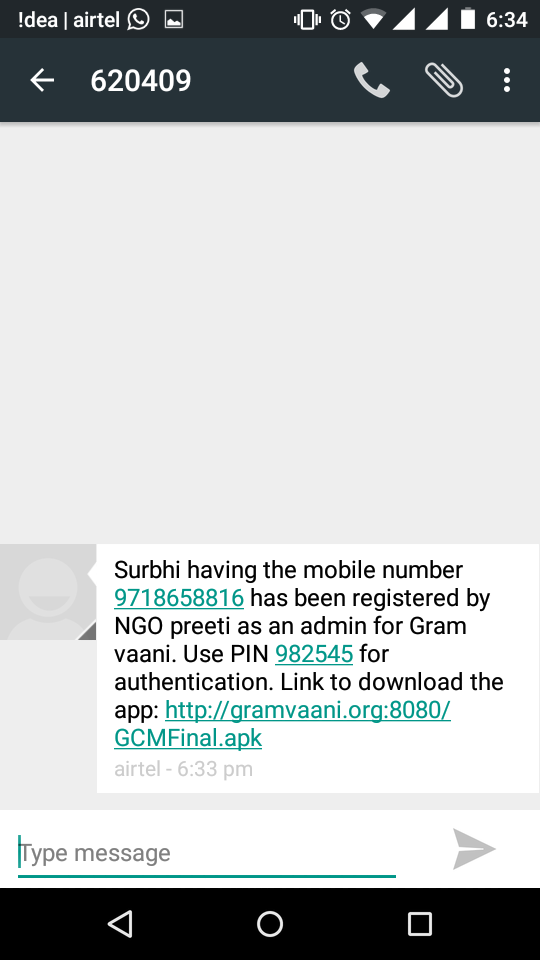
\includegraphics[scale=0.3]{authenticatemsg}
\caption{Message for Pin Authentication}
\label{fig:authenticatemsg}
\end{center}
\end{figure}

\item User can retrieve PIN by clicking on Forget PIN option.
\begin{figure}[H]
\begin{center}   
\includegraphics[scale=0.4]{Pinrecovery}
\caption{Pin Recovery}
\label{fig:pin_recovery}
\end{center}
\end{figure}

\item User will be provided with the following options.
\begin{figure}[H]
\begin{center}   
\includegraphics[scale=0.3]{Workflowapp}
\caption{Use Cases}
\label{fig:menuoptions}
\end{center}
\end{figure}

\item User can record audio by recording audio using Media Recorder.
\begin{figure}[H]
\begin{center}   
\includegraphics[scale=0.3]{Audiorecord}
\caption{Record Audio}
\label{fig:audio1}
\end{center}
\end{figure}

\item User can send instant text messages by choosing any of the below template depending upon the type of announcement.
\begin{figure}[H]
\begin{center}   
\includegraphics[scale=0.3]{Msgtemplates}
\caption{Type of Text Announcements}
\label{fig:message}
\end{center}
\end{figure}

\item Text alert of survey to be launched in the community will be sent with the specified date to inform people regarding the survey launch.
\begin{figure}[H]
\begin{center}   
\includegraphics[scale=0.4]{surveytemplate}
\caption{Announcement of Surveys}
\label{fig:message1}
\end{center}
\end{figure}

\item Text alert of upcoming camp to be organised in the community will be sent with the specified parameters to inform people. 
\begin{figure}[H]
\begin{center}   
\includegraphics[scale=0.3]{camptemplate}
\caption{Announcement of Camps}
\label{fig:message2}
\end{center}
\end{figure}


\item  Launched scheme name along with the details of scheme date and beneficiaries for that scheme will be sent to the target people to send text alerts to inform people regarding it.
\begin{figure}[H]
\begin{center}   
\includegraphics[scale=0.3]{schemetemplate}
\caption{Announcement of Govt. Schemes}
\label{fig:message3}
\end{center}
\end{figure}

\item The app users can add a new contact. The user selects the option of Add a contact on the  home screen of application. In this option, he can fill in all the details of a new contact of his community having name, contact number, gender, date of birth, contact groups and location URI.
\begin{figure}[H]
\begin{center}   
\includegraphics[scale=0.4]{Addcontact}
\caption{Add a New Contact}
\label{fig:contact1}
\end{center}
\end{figure}

\item In the above option, application user is asked for the confirmation via a diaglog box. He can either click on confirm for adding a new contact or cancel the adding of contact.
\begin{figure}[H]
\begin{center}   
\includegraphics[scale=0.4]{contactconfirm}
\caption{Confirmation Screen while Adding Contact}
\label{fig:contact2}
\end{center}
\end{figure}
 
\item  Volunteers are given this functionality for the management of contact groups. Multiple contact groups are made and managed as per the groups of the community. It helps in easy dissemination of information to the relevant audience.
\begin{figure}[H]
\begin{center}   
\includegraphics[scale=0.4]{addgroup}
\caption{Add a New Contact Group}
\label{fig:group1}
\end{center}
\end{figure}

\item Application user can view the active survey of the GramVaani Server corresponding to the application instance.
\begin{figure}[H]
\begin{center}   
\includegraphics[scale=0.4]{launchsurvey}
\caption{List of Active Surveys}
\label{fig:viewlaunchsurvey}
\end{center}
\end{figure}

\item Application user can view a particular survey with all the survey questions along with the type of question. One can also listen the audio prompt of each survey question.
\begin{figure}[H]
\begin{center}   
\includegraphics[scale=0.3]{surveyques}
\caption{View a Particular Survey}
\label{fig:viewsurvey}
\end{center}
\end{figure}

\item  Application user can choose the target people among the gram vaani groups, his phone callers and  Mobile Vaani instance callers.
\begin{figure}[H]
\begin{center}   
\includegraphics[scale=0.4]{sendoptions}
\caption{Choose Contact Options to Launch}
\label{fig:contactoptions}
\end{center}
\end{figure}

\item Multiple Gram Vaani contact groups can be choosen as the target audience.
\begin{figure}[H]
\begin{center}   
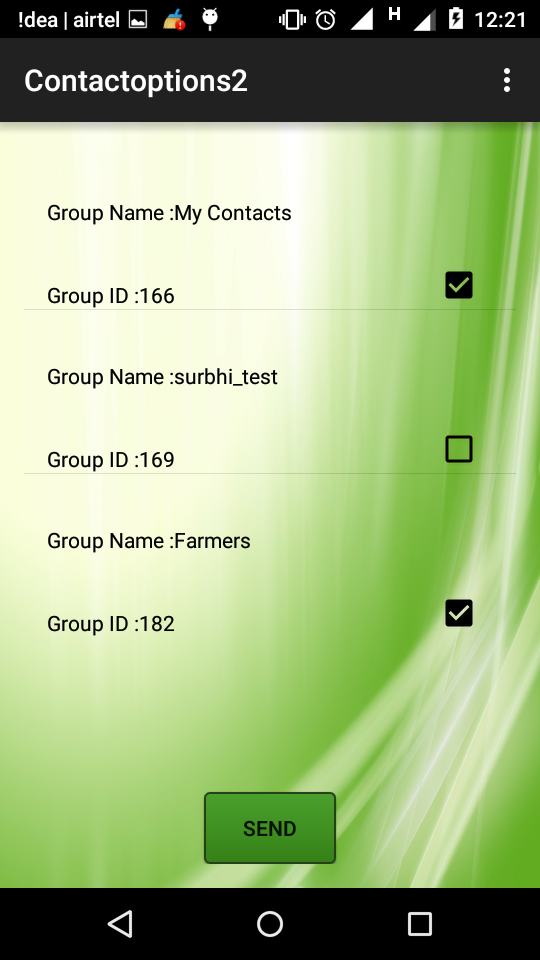
\includegraphics[scale=0.3]{contactgroups}
\caption{GV Contact Groups}
\label{fig:contactgroups}
\end{center}
\end{figure}

\item Multiple phone contacts can be choosen as the target people.
\begin{figure}[H]
\begin{center}   
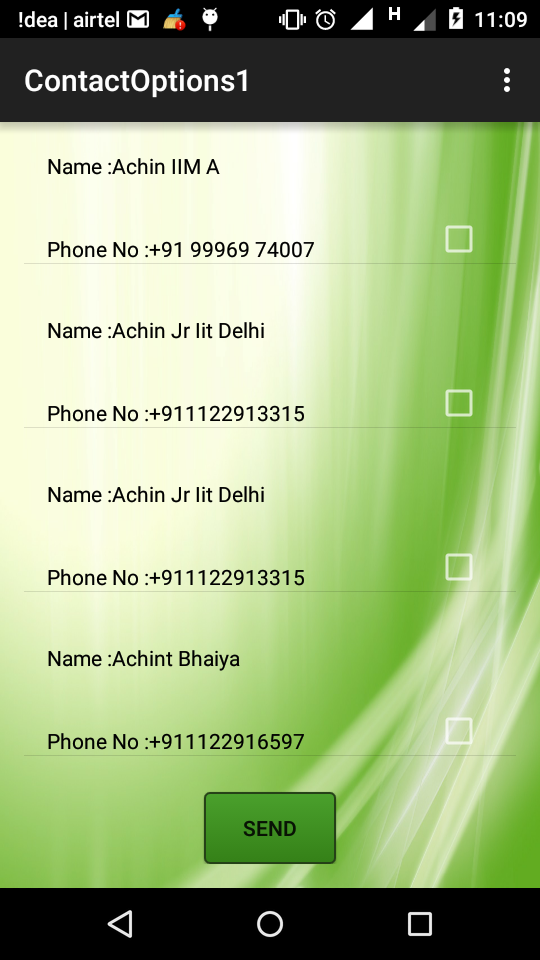
\includegraphics[scale=0.4]{phonecontacts}
\caption{Phone Contacts}
\label{fig:phonecontacts}
\end{center}
\end{figure}

\item Some quick options are provided on the application which are available across all activities. Application  user can navigate across these options.
\begin{figure}[H]
\begin{center}   
\includegraphics[width=0.8\textwidth]{Actionbaroptions}
\caption{Options on Menu Bar}
\label{fig:menubar}
\end{center}
\end{figure}

\end{enumerate}





\chapter{Screenshots of the Web Portal}

\begin{enumerate}
\item Home Page of the Web Portal for NGO's Registration and other functionalities
\begin{figure}[here]
\begin{center}   
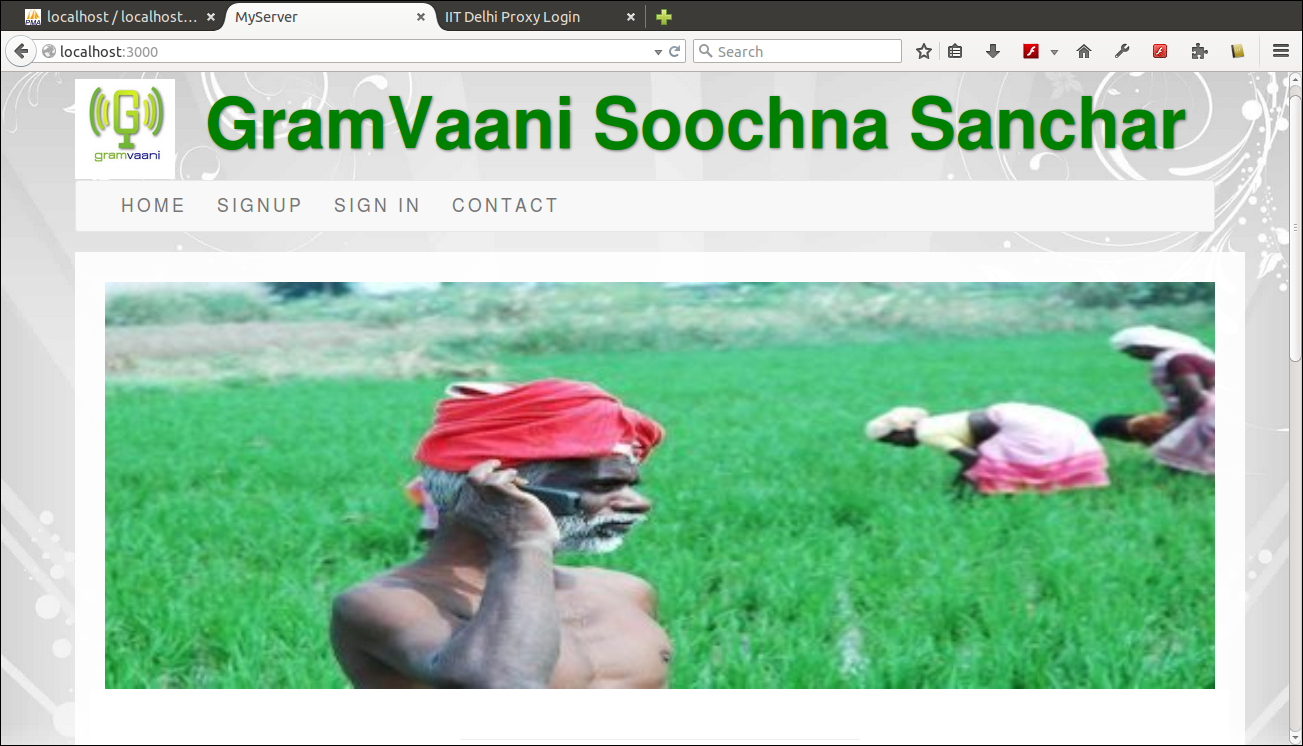
\includegraphics[scale=0.3]{w1}
\caption{GramVaani Soochna Sanchar Home Page}
\label{fig:w1}
\end{center}
\end{figure}


\item NGO's Login Page
\begin{figure}[here]
\begin{center}   

\includegraphics[scale=0.3]{w10}
\caption{NGO's Login Page}
\label{fig:w10}
\end{center}
\end{figure}



\item Use cases provided to the NGO users
\begin{figure}[here]
\begin{center}   

\includegraphics[scale=0.3]{w14}
\caption{Use Cases of NGO Personnel}
\label{fig:w14}
\end{center}
\end{figure}



\item Web Online form for Admins Registration and Authentication
\begin{figure}[here]
\begin{center}   
\includegraphics[scale=0.3]{w15}
\caption{Admin's Registration Form}
\label{fig:w15}
\end{center}
\end{figure}




\item NGO Personnel can launch a particular survey for a particular district.
\begin{figure}[here]
\begin{center}   
\includegraphics[scale=0.3]{w16}
\caption{Launch Survey in a District}
\label{fig:w16}
\end{center}
\end{figure}


\item NGO Personnel can view all the active surveys along with viewing current responses and survey questions.
\begin{figure}[here]
\begin{center}   
\includegraphics[scale=0.3]{w13}
\caption{View Active Surveys}
\label{fig:w13}
\end{center}
\end{figure}


\item NGO Personnel can view the responses of the active survey.
\begin{figure}[here]
\begin{center}   
\includegraphics[scale=0.3]{w11}
\caption{View Active Survey Responses}
\label{fig:w11}
\end{center}
\end{figure}


\item NGO Personnel can view the text questions of the active survey.
\begin{figure}[here]
\begin{center}   
\includegraphics[scale=0.3]{w12}
\caption{View Active Survey Questions}
\label{fig:w12}
\end{center}
\end{figure}
 
\end{enumerate}

\chapter{Screenshot of the GramVaani GUI Instance}

\begin{enumerate}

\item GramVaani Graphical Web Portal Instance
\begin{figure}[here]
\begin{center}   
\includegraphics[scale=0.3]{gvinstance1}
\caption{GramVaani Web Instance}
\label{fig:gvinstance1}
\end{center}
\end{figure}

\end{enumerate}
















\end {document}
	